\chapter{User Manual}

\section{Introduction}

The purpose of my program is to act as a skateboarding progress tracker and personal assistant. The program was built to aid skateboarding progress, maximise physical performance and enhance muscle memory by reminding the user of newly learnt tricks. The skateboard progress tracker also caters for the users skateboarding buying needs as it includes its very own skateboard part review hub. The integrated Google maps keeps a store of all of the skateparks and skate spots in the world, which skaters using the program can add to.

The intended audience of my program is currently purely for my client; however in the future, once a multi-user platform has been integrated the intended audience will be for the whole skating community.

As the skateboard progress tracker is still an uncompleted program, some of the functionality is not currently available in a graphical user interface format and not all of the validation is fully functional.

Currently, the version of the skateboard progress tracker includes a personalised profile tab where you can change the profile picture, email address and name to your own personal information. The tricks tab contains a table with a list of all the tricks in the database. You may delete tricks from your database by selecting the desired row and pressing delete. Another function on the tricks tab is the ability to add a trick to the database. With an easy to fill, side form that appears when 'add trick' is selected.This tab is used to keep a record of all the tricks that the user can do. The skatepark tab contains a customisable Google maps object which allows you to add and remove skateparks. This tab is used so that the user can plan on visiting new skateparks that they have never been to before. The review tab contains a table which displays all the reviews in the database. Functionality with the graphical user interface will be integrated in the next version of the program. The support tab allows the user to report any problems with the program, and request any additional functionality that they wish me to implement.





\section{Installation}

\textbf{System Requirements}

Before installing, your computer must meet the system requirements. As discussed in the analysis and design section (Subsections 1.7.1  and 2.3 respectively) I am developing this program for my client, therefore the system is built to run on:

\begin{itemize}
    \item 15.6" HD 1366x768 Screen
    \item i5-2450M Dual Core Processor (Sandy Bridge) 2.5GHz (overclocked to 3.1GHz) 3MB Cache
    \item 8GB DDR3 RAM
    \item 500GB HDD Memory
    \item Intel HD3000 Graphics Card
    \item Windows 7 Operating System
\end{itemize}

My program has been tested, and works on Windows 7 and Vista. Although the program hasn't been tested on Mac computers or windows 8, the program should still work fine as long as the required programs are installed correctly as discussed below.




\subsection{Prerequisite Installation}


\subsubsection{Installing Python 3.4}

To install Python 3.4, first you must go to the web page: \url{https://www.python.org/downloads/release/python-340/}. The following web page will be presented.

\begin{figure}[H]
    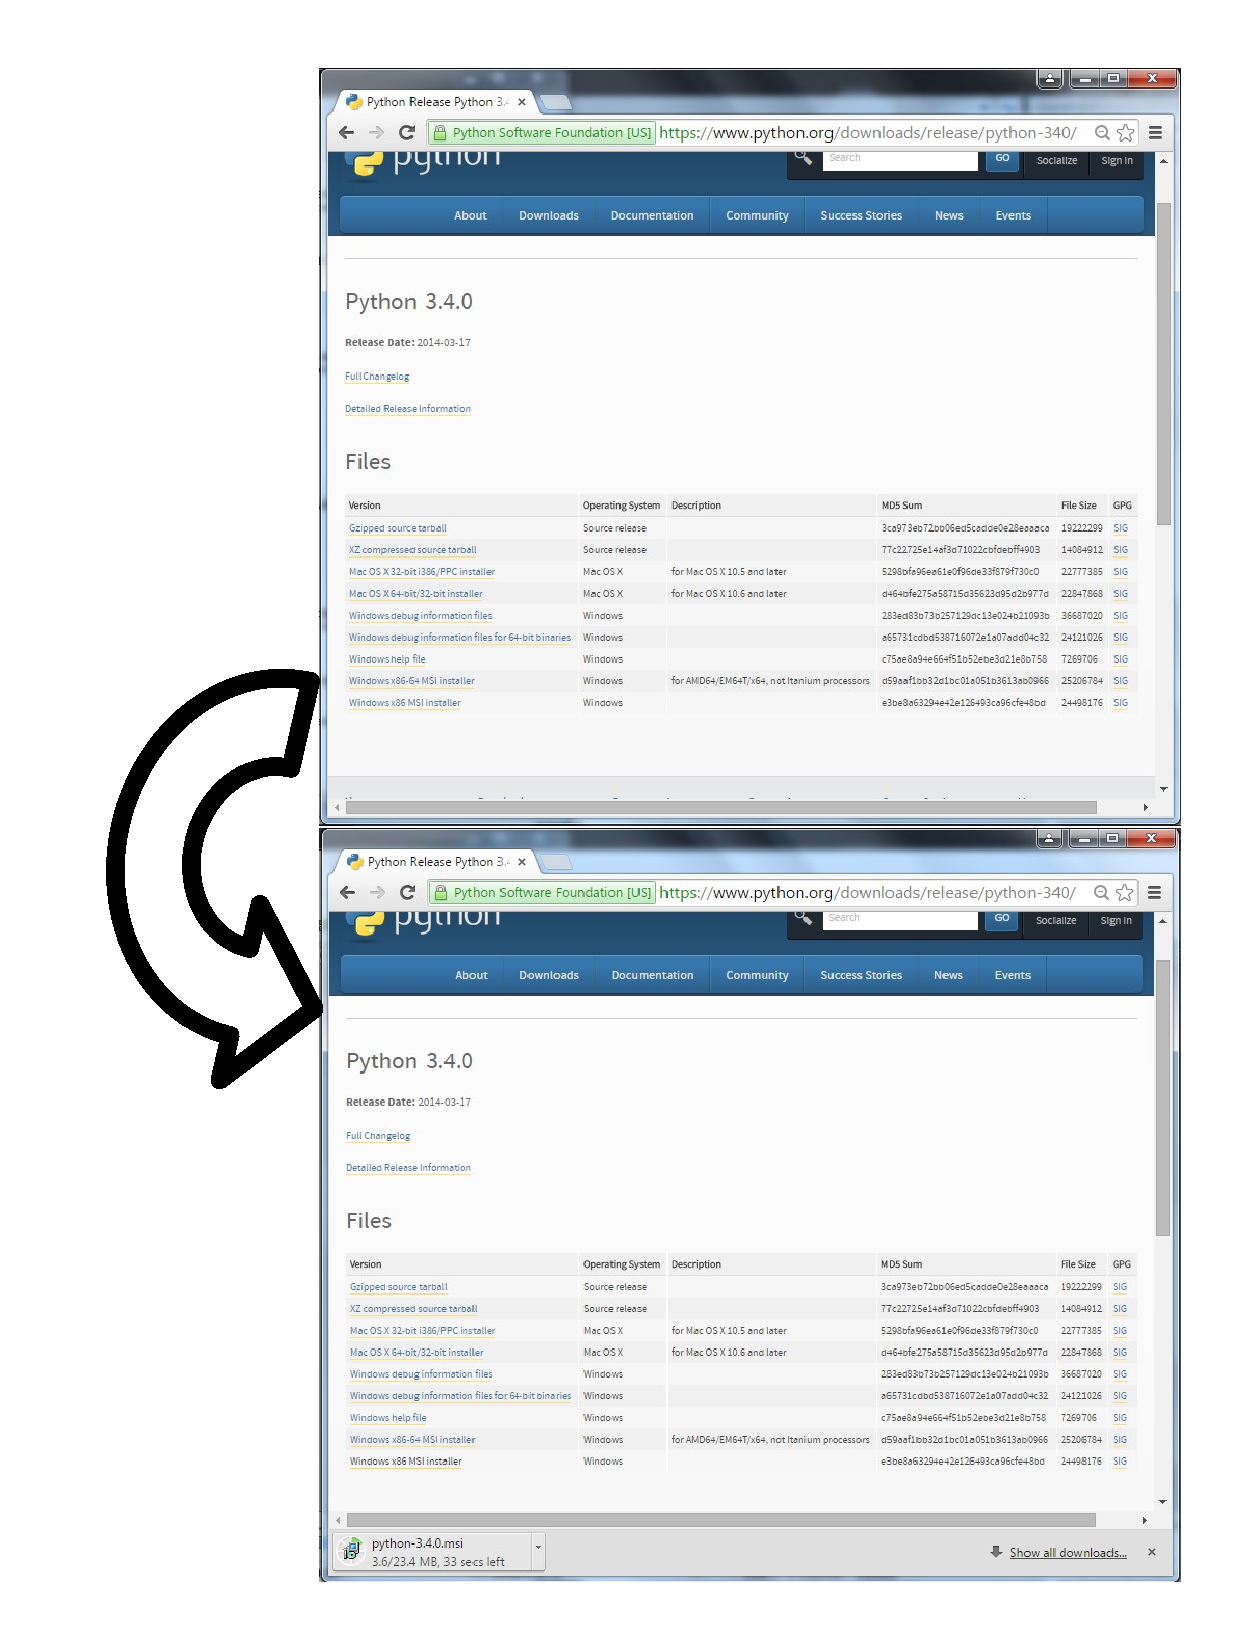
\includegraphics[width=\textwidth]{./Manual/Images/DownloadingPython.pdf}
    \caption{Downloading Python 3.4} \label{fig:DownloadingPython}
\end{figure}

Select the appropriate installer for your computer. Once the installer has been downloaded, click on the downloaded file.

\begin{figure}[H]
    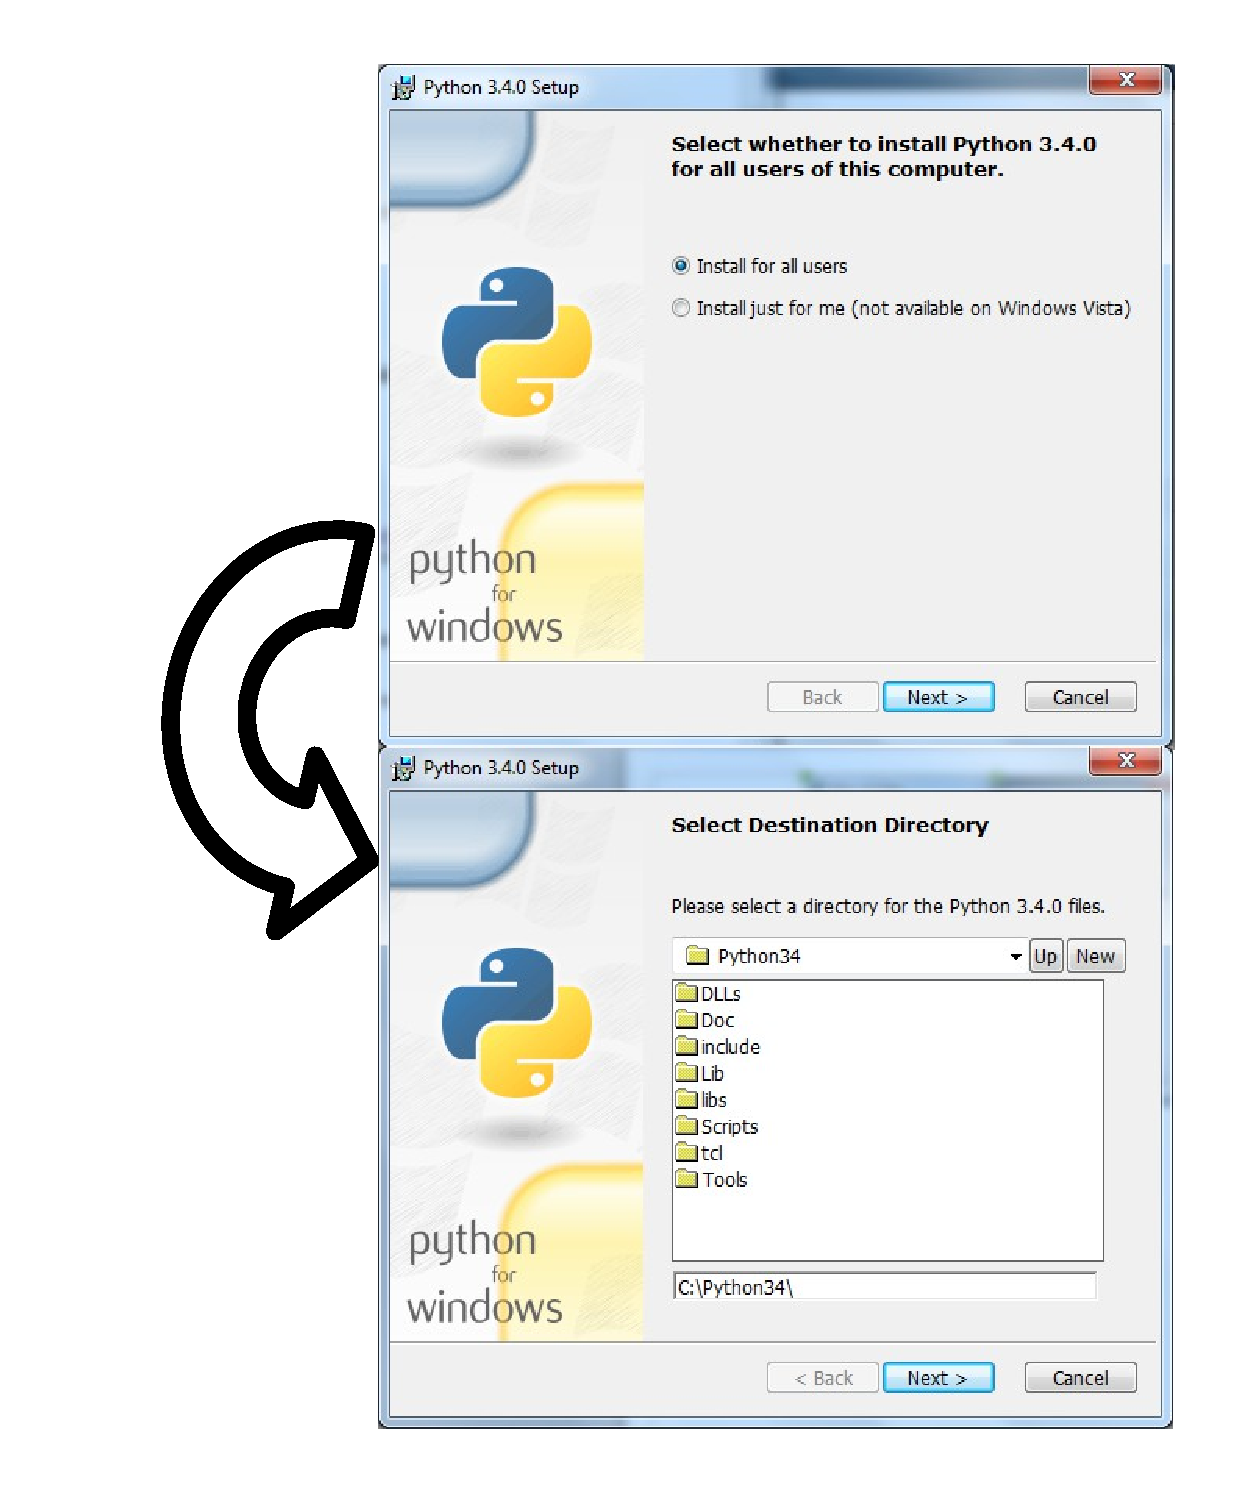
\includegraphics[width=\textwidth]{./Manual/Images/InstallingPython.pdf}
    \caption{Installing Python 3.4} \label{fig:InstallingPython}
\end{figure}

The figure above shows the python set up process. Click next on both installer windows and wait for the installing process to complete. After the installer has finished, python 3.4 will now be installed, and ready to use on your computer.

\subsubsection{Installing PyQt 4}

To install PyQt 4, first you must go to the web page: \url{http://www.riverbankcomputing.co.uk/software/pyqt/download}. The following web page will be presented.

\begin{figure}[H]
    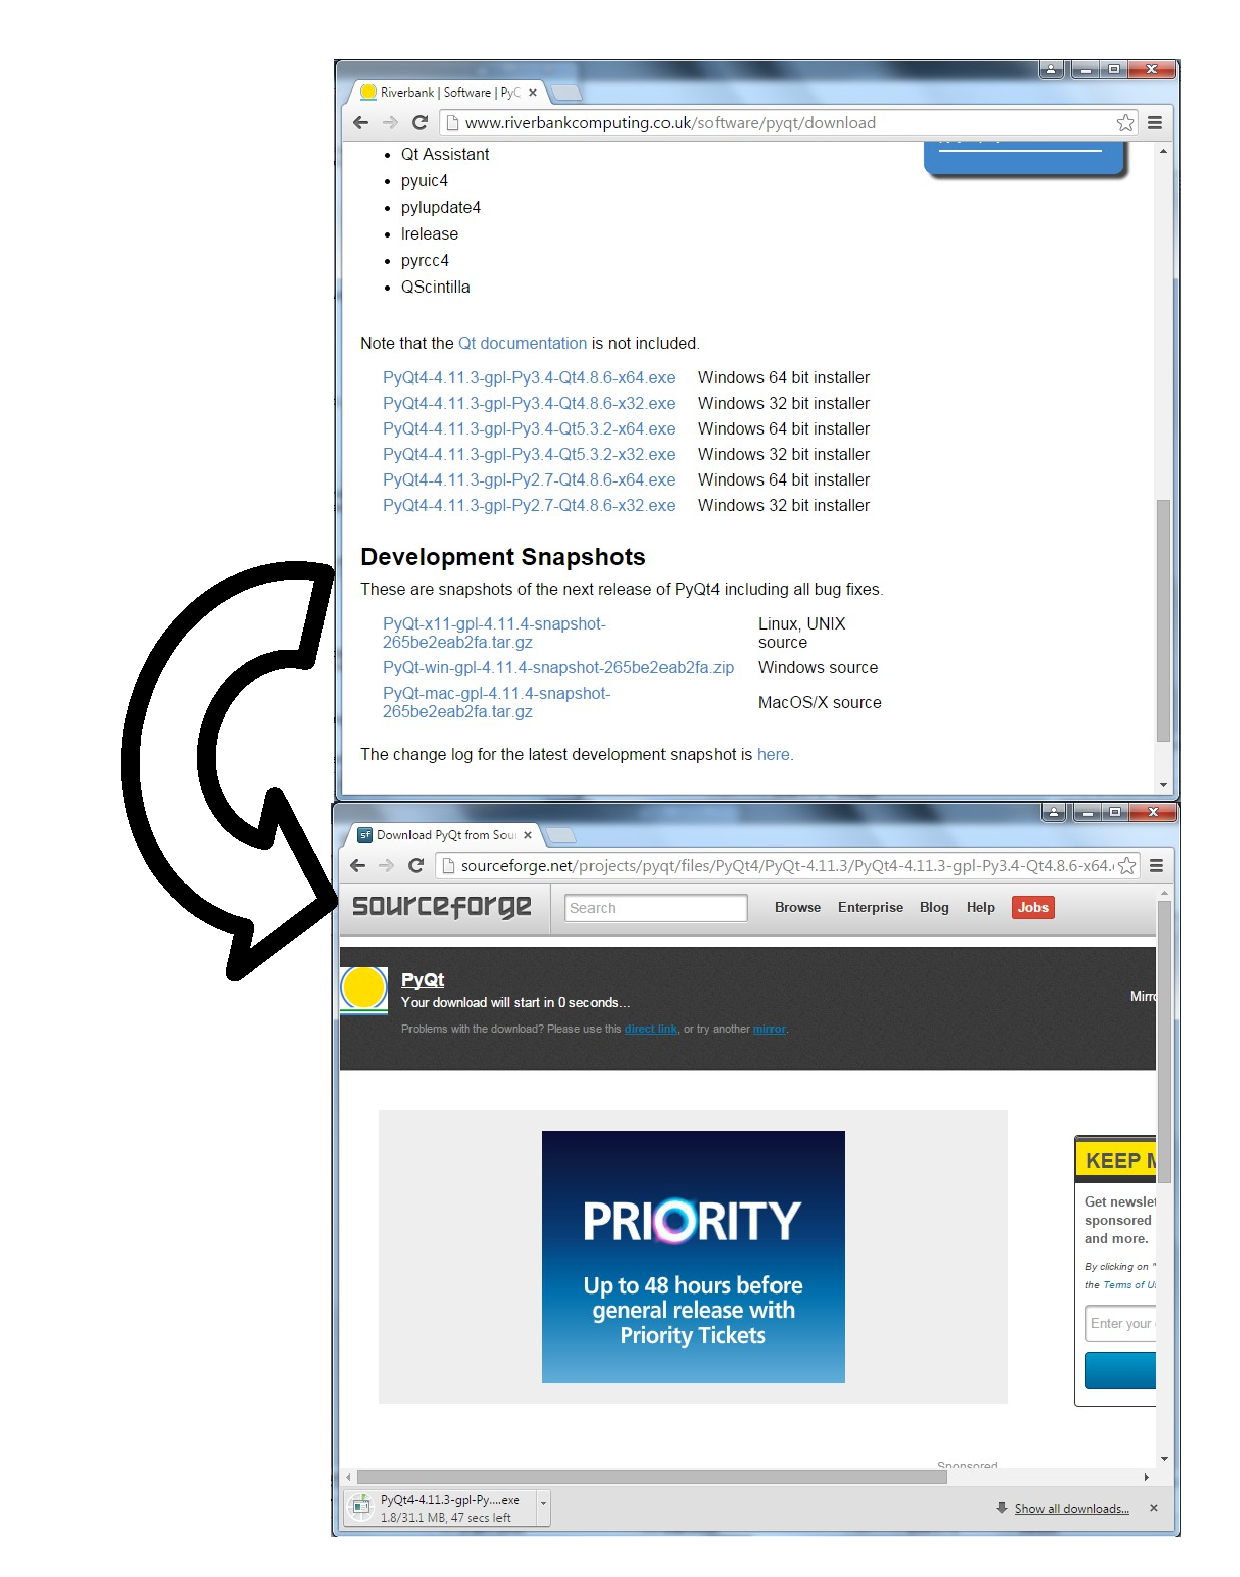
\includegraphics[width=\textwidth]{./Manual/Images/DownloadingPyQt.pdf}
    \caption{Downloading PyQt} \label{fig:DownloadingPyQt}
\end{figure}

Select the appropriate installer of PyQt 4 for your computer. Once the installer has been downloaded, click on the downloaded file.

\begin{figure}[H]
    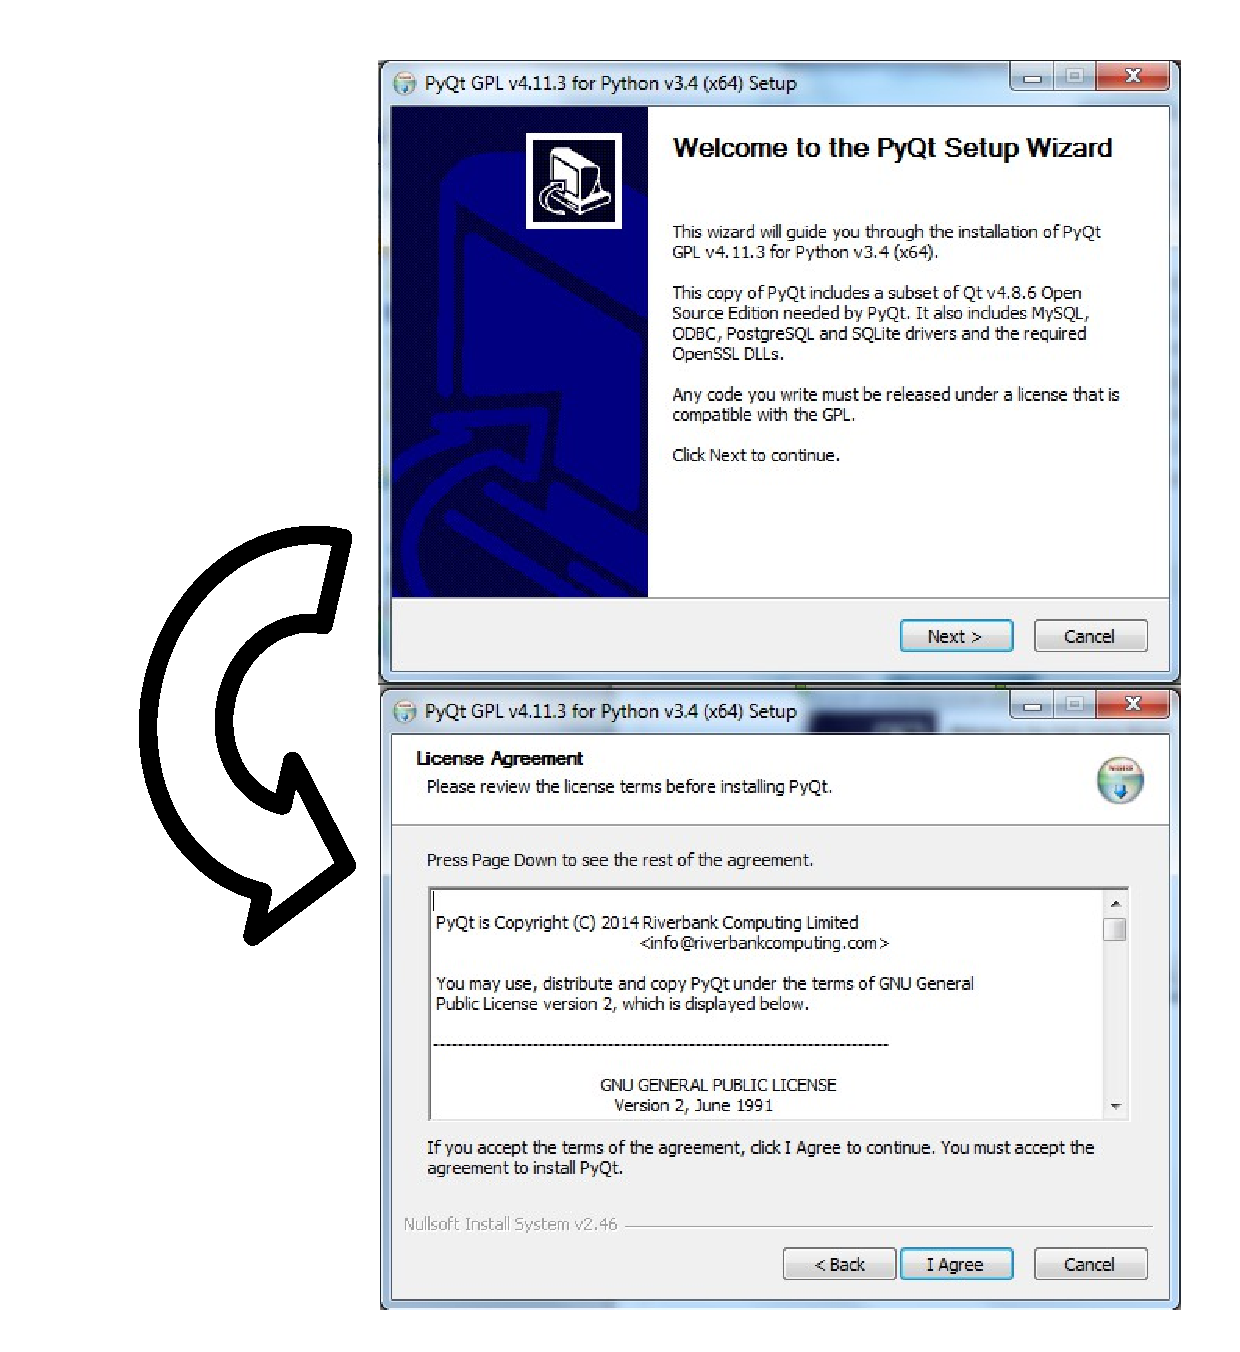
\includegraphics[width=\textwidth]{./Manual/Images/InstallingPyQt.pdf}
    \caption{Installing PyQt 4} \label{fig:InstallingPyQt}
\end{figure}

\begin{figure}[H]
    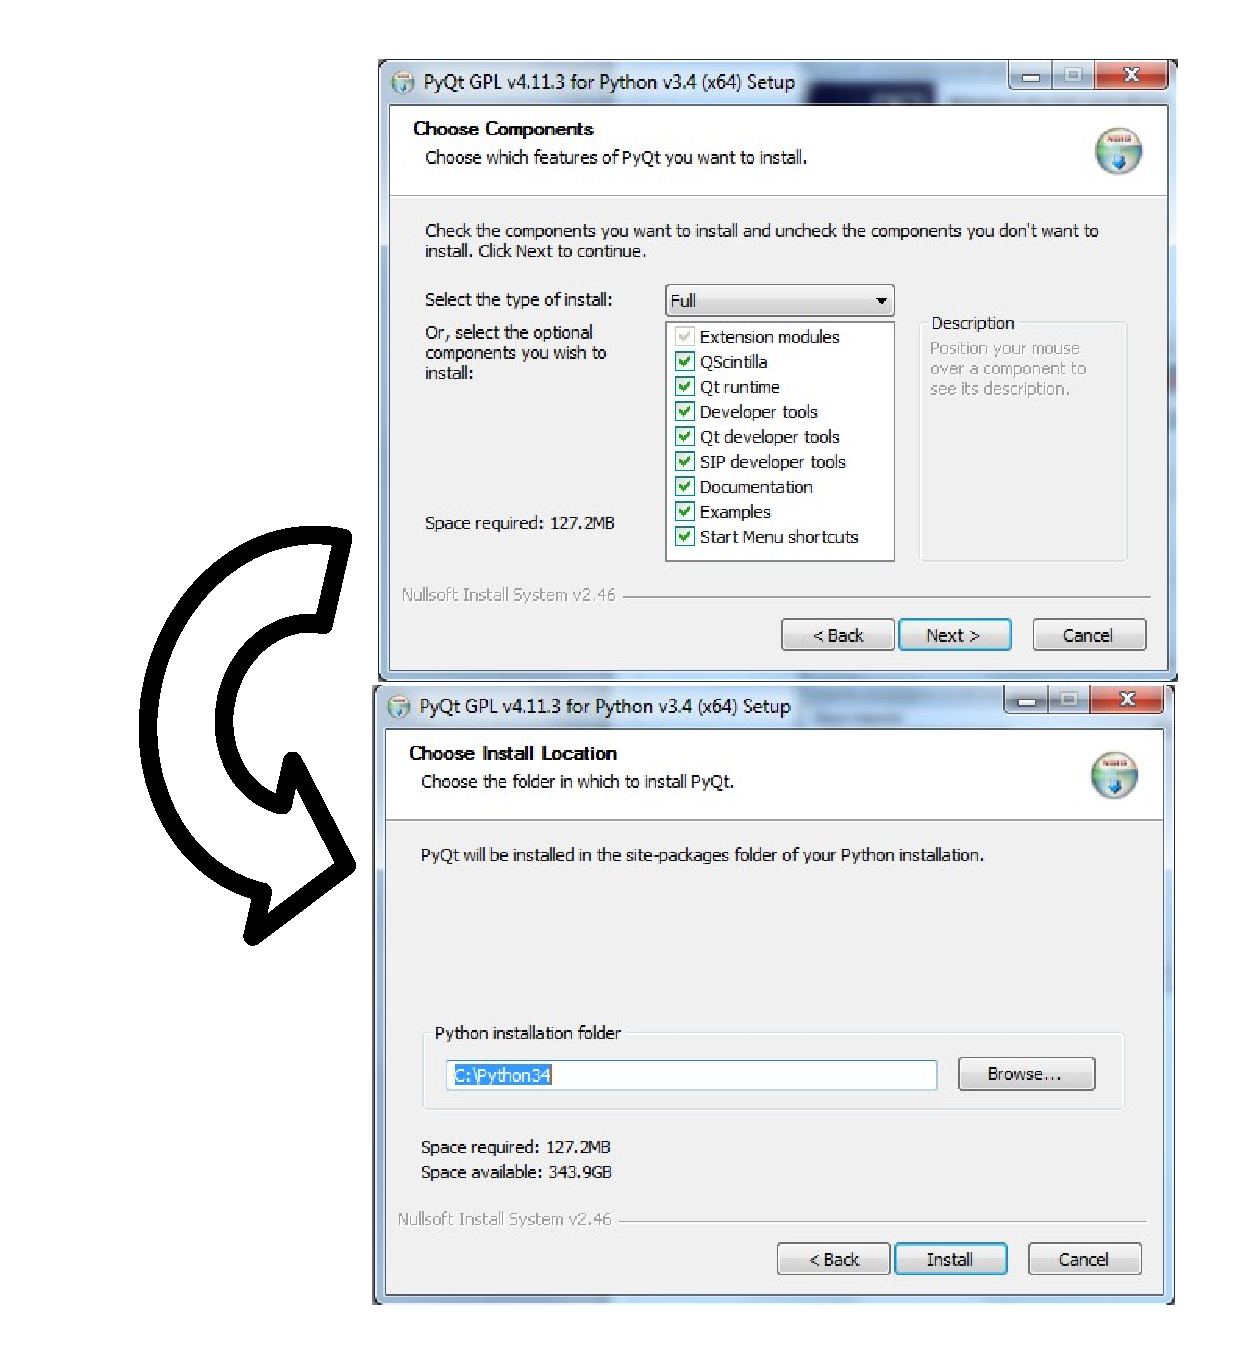
\includegraphics[width=\textwidth]{./Manual/Images/InstallingPyQtp2.pdf}
    \caption{Installing PyQt 4 Part 2} \label{fig:InstallingPyQtP2}
\end{figure}

The figure above shows the PyQt set up process. Click 'Next' followed by 'I agree', followed by 'Next' and finally 'Install'. Wait for the installing process to complete. Once the installer has finished, PyQt4 will now be installed, and ready to use on your computer.

\subsection{System Installation}

To install the system go to my personal github page and find the Comp4 repository (\url{http://www.github.com/BenKeppie}). Click on the download zip button and then save the file in an appropriate place on your hard drive.

\begin{figure}[H]
    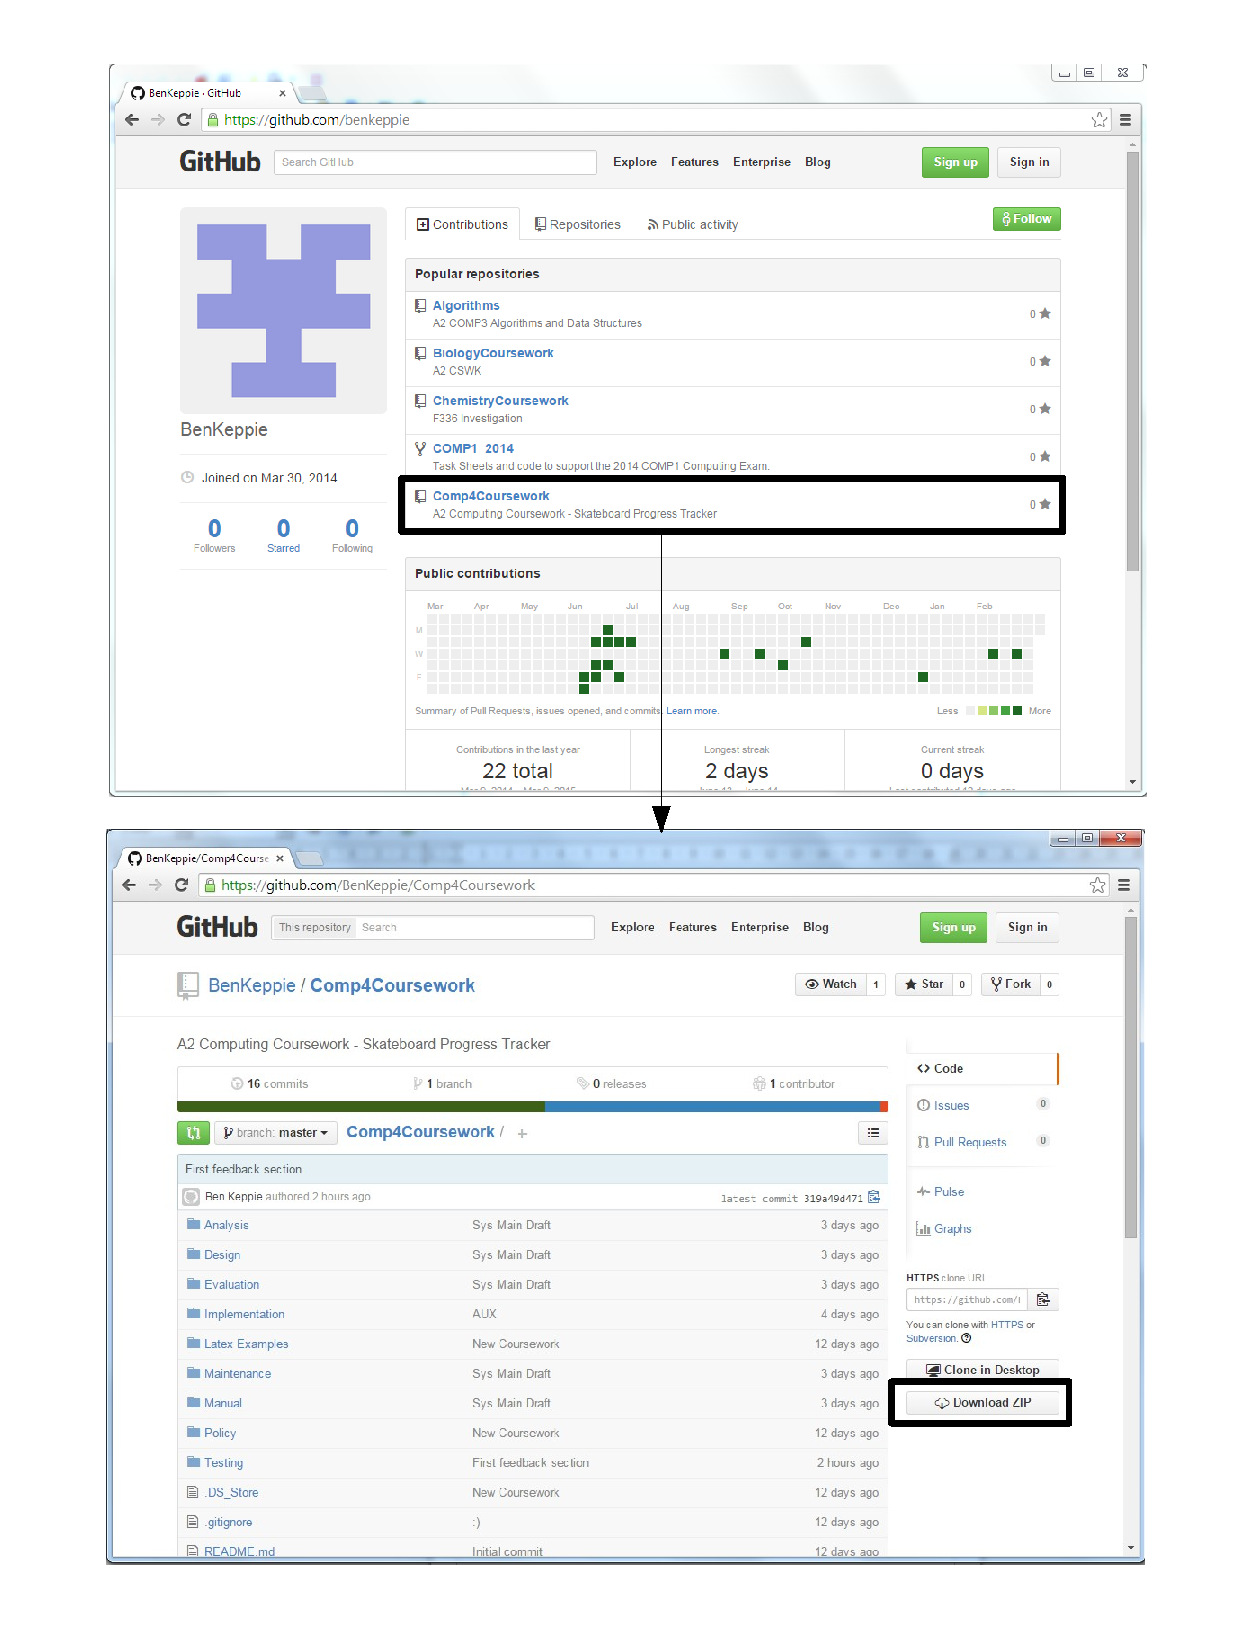
\includegraphics[width=\textwidth]{./Manual/Images/BenGithub.pdf}
    \caption{Downloading Skateboarding Progress Tracker Application} \label{fig:Downloading Program}
\end{figure}

To extract the files to a usable form you will need to extract the zip file. To do this you need to find the downloaded zip file, right click on it and save the extracted folder in an appropriate destination.

\begin{figure}[H]
    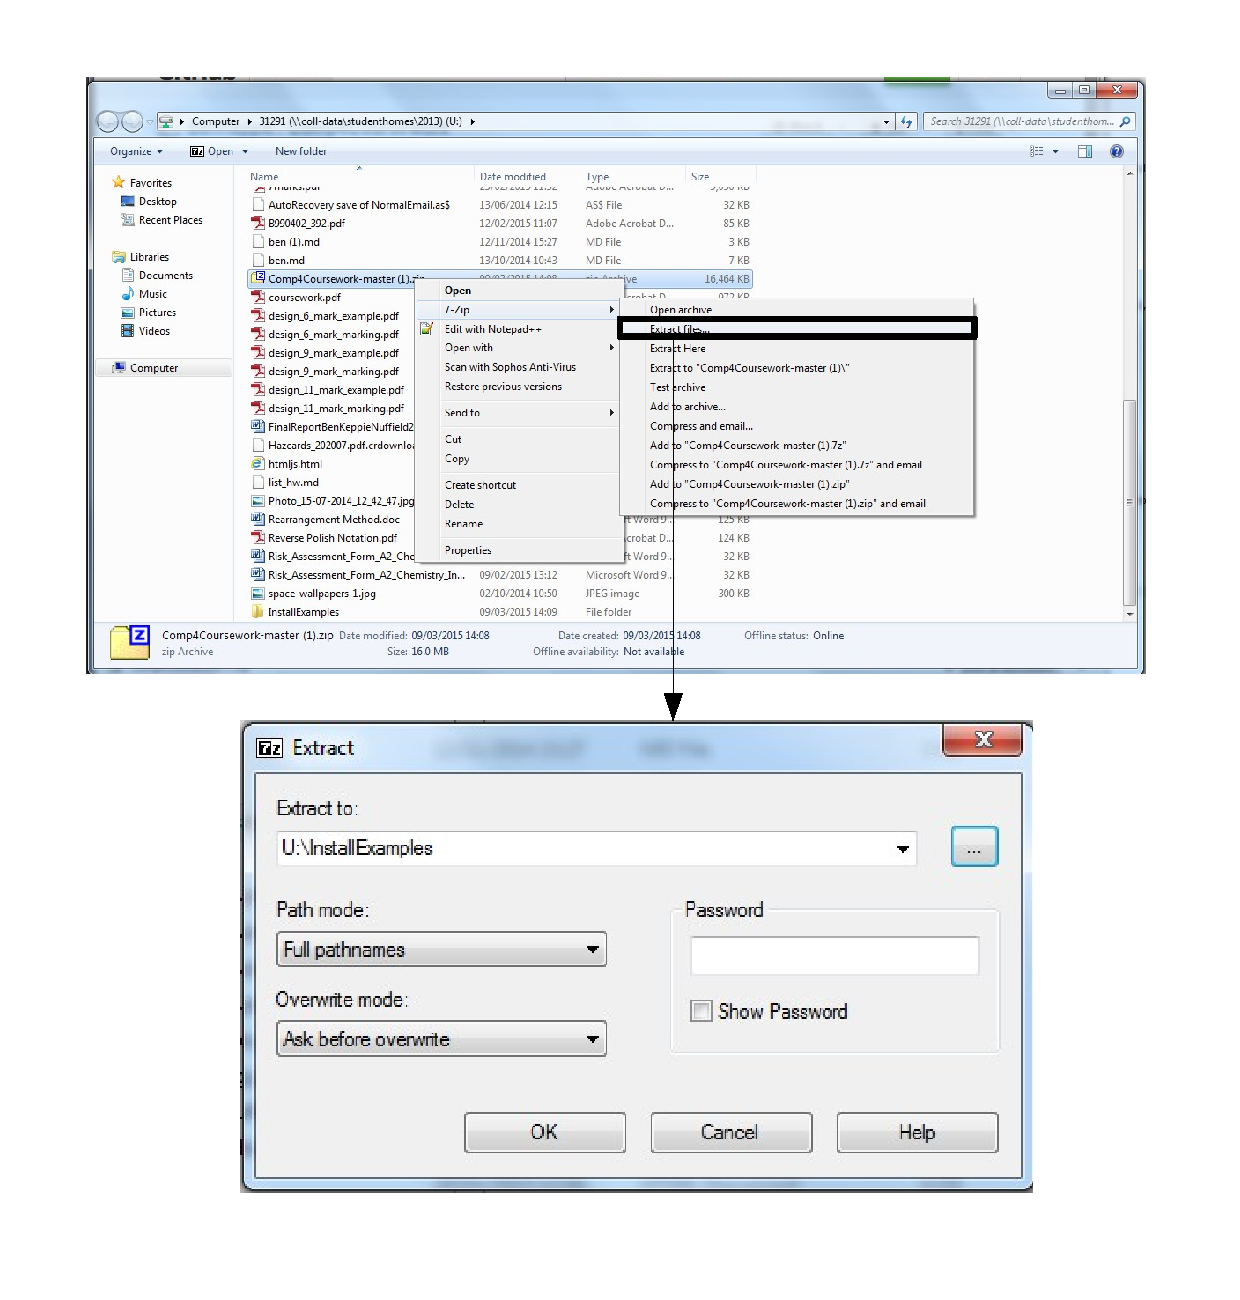
\includegraphics[width=\textwidth]{./Manual/Images/ExtractZIP.pdf}
    \caption{Extracting the zip File} \label{fig:Extracting ZIP}
\end{figure}

The system is now available to run as long as the appropriate programs discussed above are installed.


\subsection{Running the System}

To run the system, open the file location that you extracted the zip file to previously and navigate into the folder 'Implementation' and then click on the file 'main\_window.pyw', the program will now be loading, as shown by the start up of the splash screen.

\begin{figure}[H]
    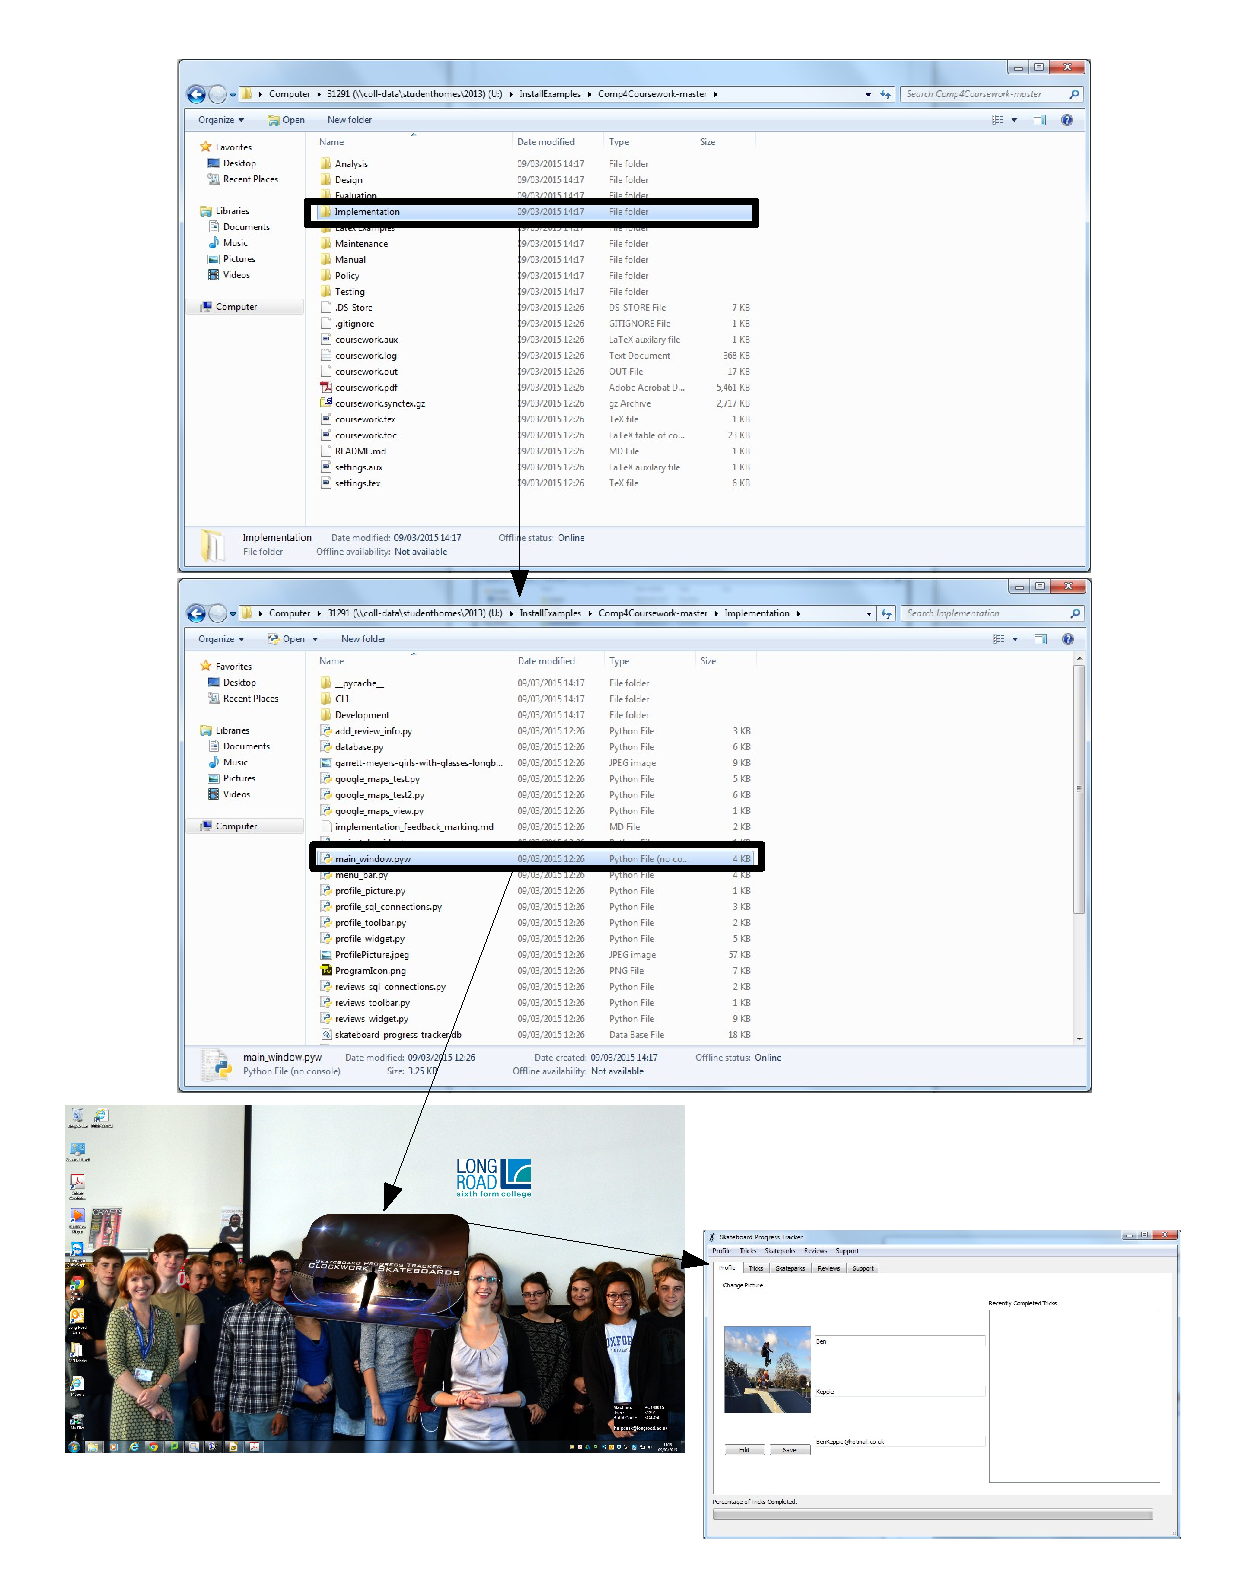
\includegraphics[width=\textwidth]{./Manual/Images/RunningProgram.pdf}
    \caption{Starting up the program} \label{fig:Running Program}
\end{figure}







\section{Tutorial}

\subsection{Introduction}

This tutorial will talk you through how to navigate and operate the Skateboard Progress Tracker application, with annotated screen shots.

\subsection{Assumptions}

I am assuming that the user has basic computer operating skills. These include: Using a mouse and keyboard. Apart from that, to use the Skateboard Progress Tracker, you need no prior knowledge of the system, or how it works in order to operate the program.

\subsection{Tutorial Questions}

\subsubsection{How Do I Change My Profile Picture?}

\begin{figure}[H]
    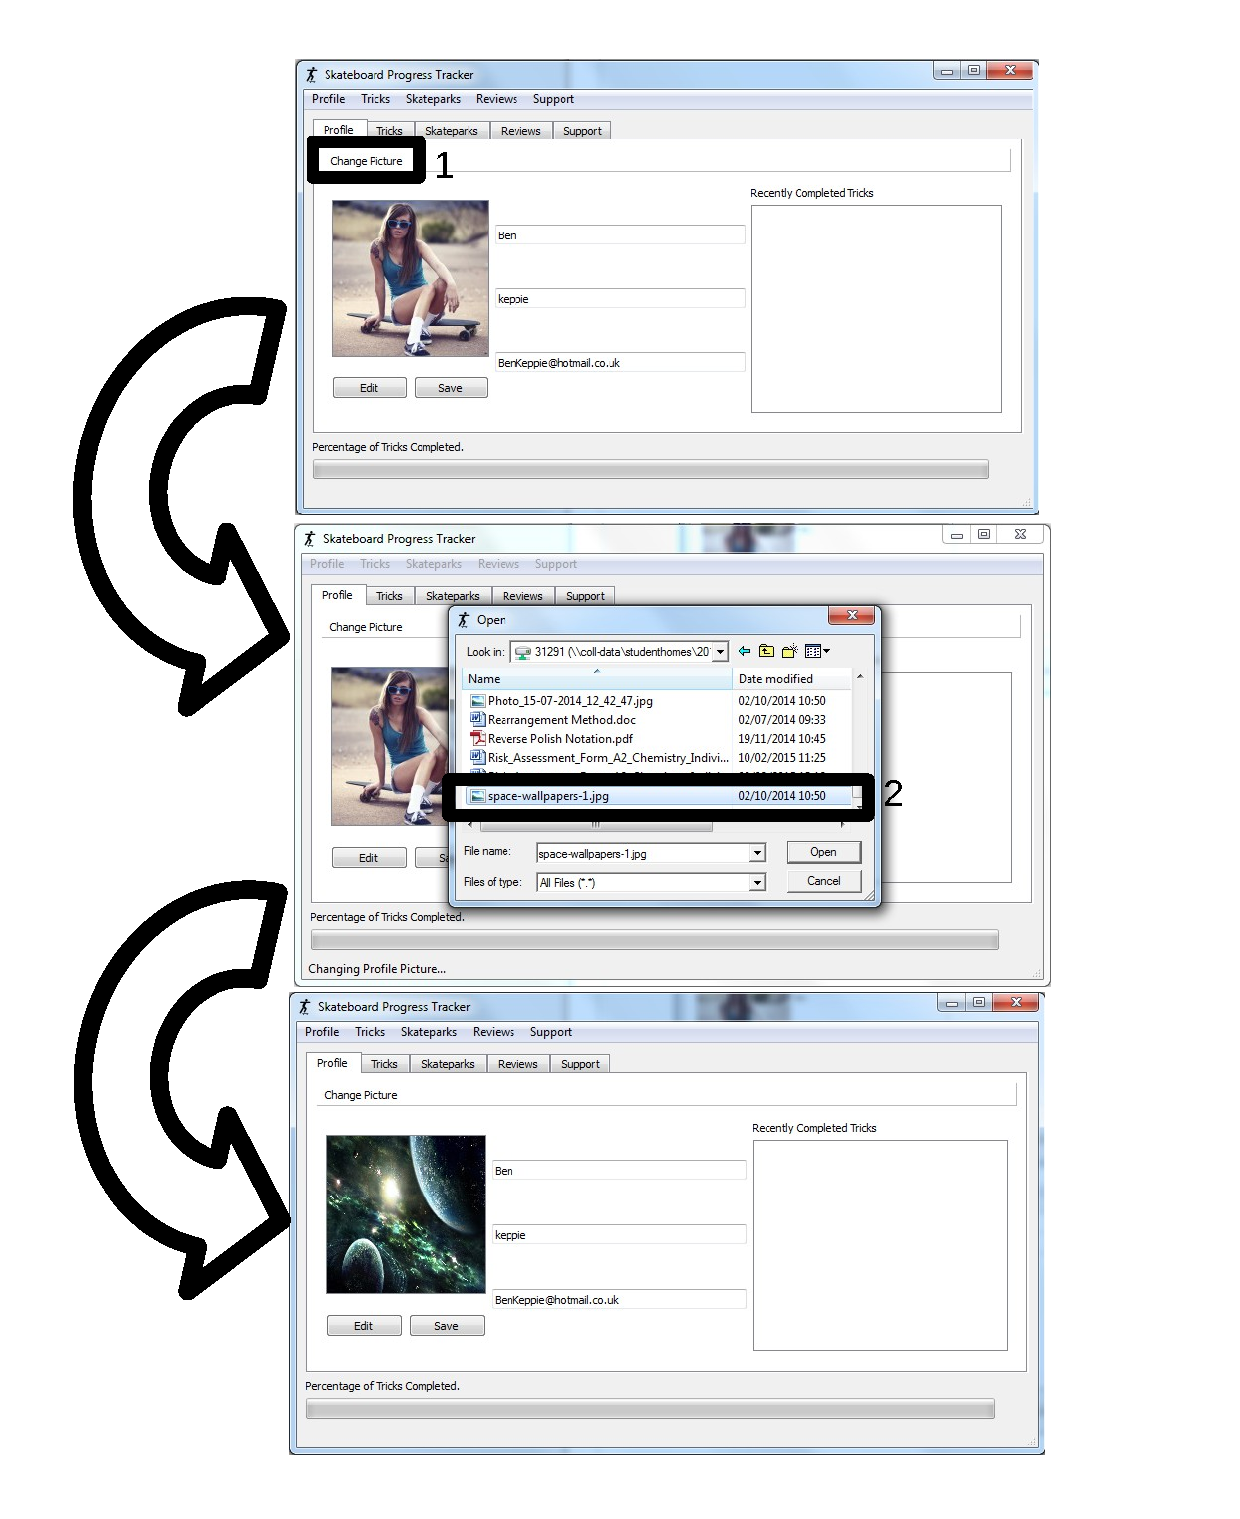
\includegraphics[width=\textwidth]{./Manual/Images/SaveProfilePicture.pdf}
    \caption{Changing The Profile Picture} \label{fig:Change Profile Picture}
\end{figure}

The figure above shows you a step by step graphical tutorial in how to change your profile picture. Below, a text tutorial will guide you through the numbers represented on the figure.
\begin{enumerate}
\item Click on the 'Change Picture' button on the profile tool bar.
\item A pop-up will appear, allowing you to chose a JPEG image to use as your profile picture. Double click on an appropriate JPEG image, this will save the profile picture and change the image on your profile.
\end{enumerate}


\subsubsection{How Do I Change My Profile Name?}

\begin{figure}[H]
    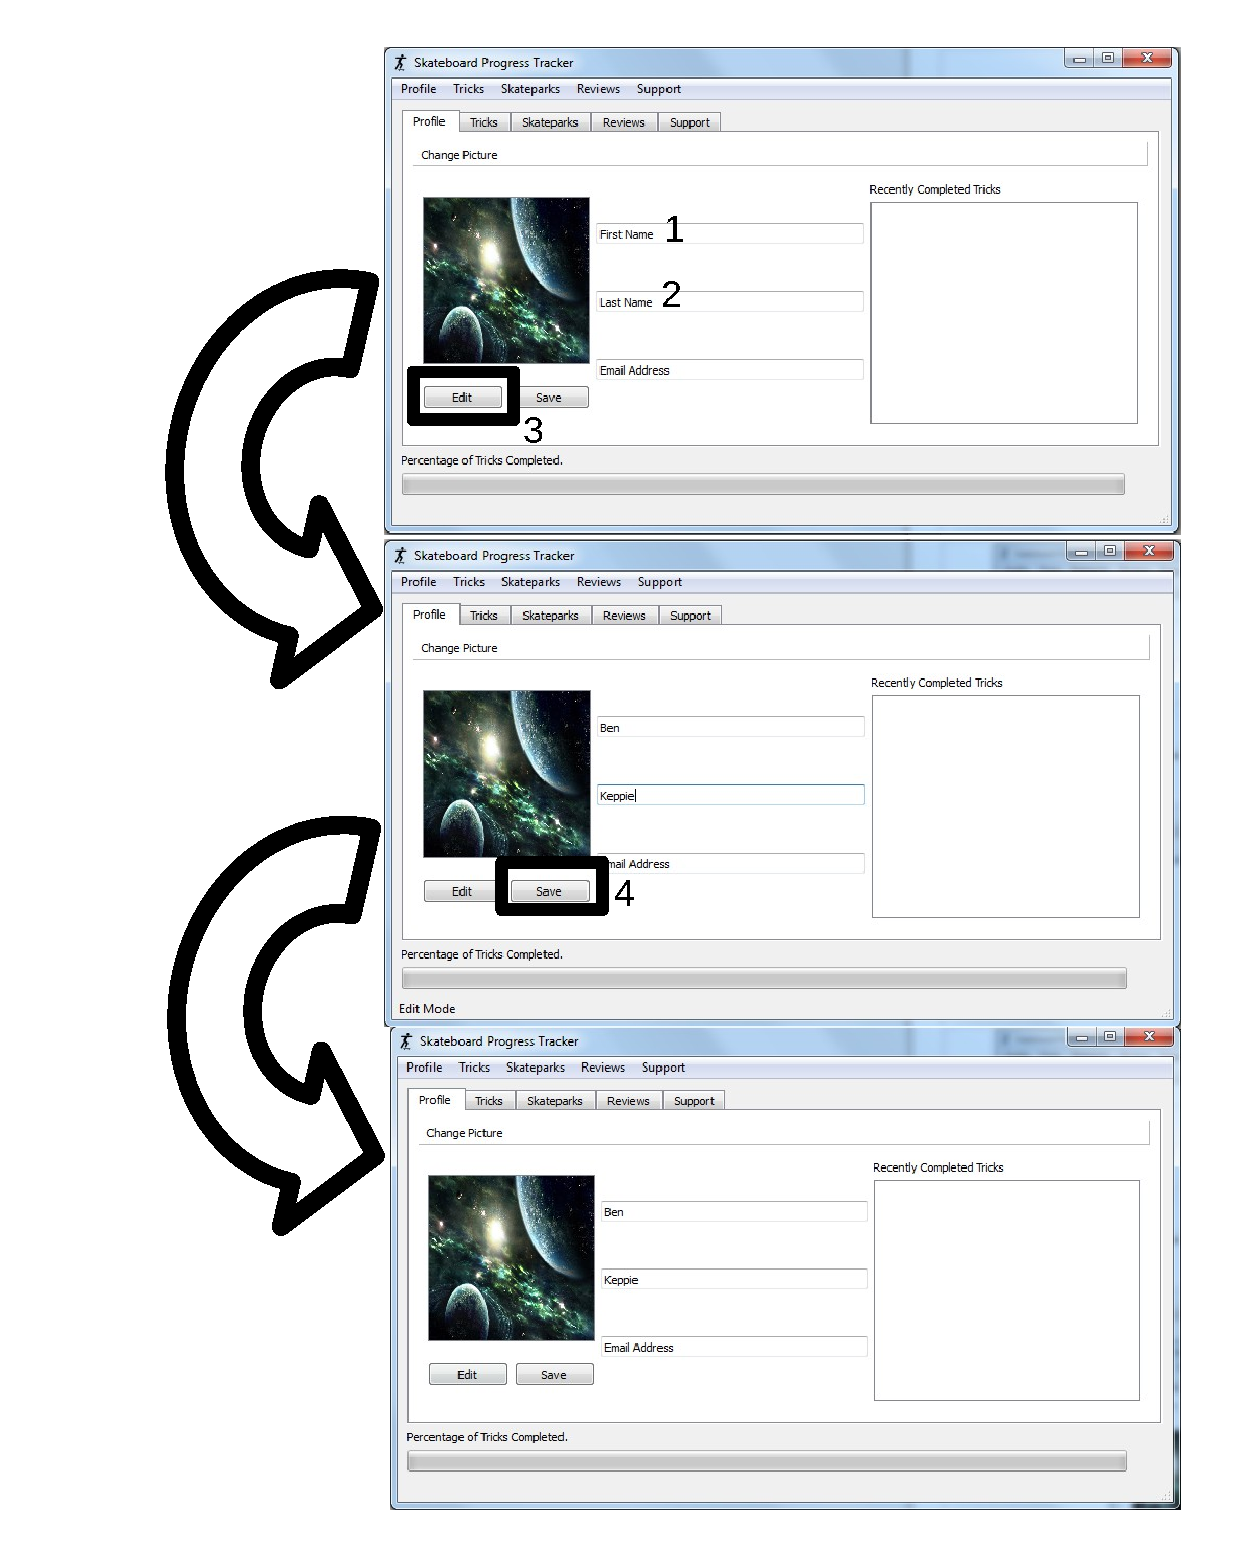
\includegraphics[width=\textwidth]{./Manual/Images/ChangeName.pdf}
    \caption{Changing The Profile name} \label{fig:Change Name}
\end{figure}

The figure above shows you a step by step graphical tutorial in how to change your profile picture. Below, a text tutorial will guide you through the numbers represented on the figure.

\begin{enumerate}
\item This is the field available to put your First Name in.
\item This is the field available to put your Last Name in.
\item Click edit to enter edit mode, which allows you to edit your name. Once this is done, enter your name in the fields.
\item Once you have changed your name, save the changes by clicking save.
\end{enumerate}

\subsubsection{How Do I Change My Profile Email Address?}

\begin{figure}[H]
    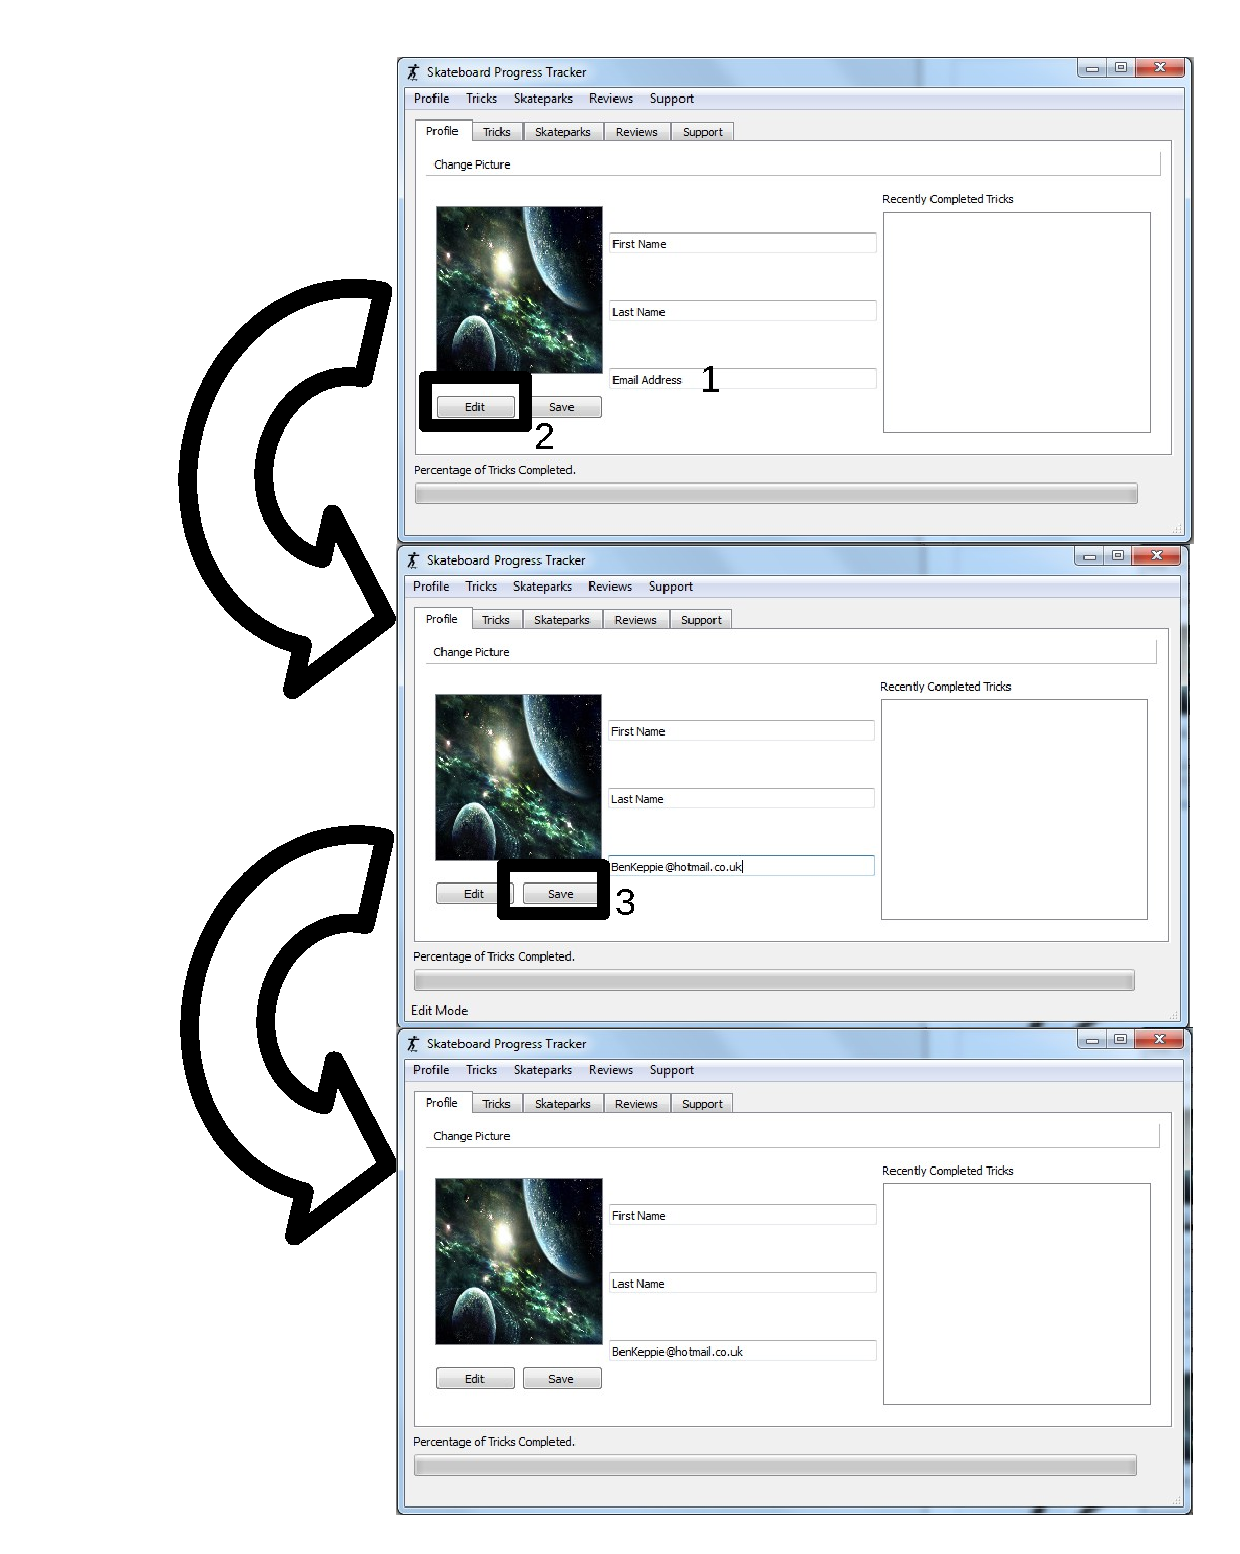
\includegraphics[width=\textwidth]{./Manual/Images/ChangeEmail.pdf}
    \caption{Changing The Profile Email Address} \label{fig:Change Email}
\end{figure}

The figure above shows you a step by step graphical tutorial in how to change your profile picture. Below, a text tutorial will guide you through the numbers represented on the figure.

\begin{enumerate}
\item This field is available to put your email address in.
\item Click edit to enter edit mode, which allows you to change your email. Once this is done, enter your email address in the appropriate field.
\item Once you have changed your email address, save the changes by clicking save.
\end{enumerate}

\subsubsection{How Do I Add a Trick?}

\begin{figure}[H]
    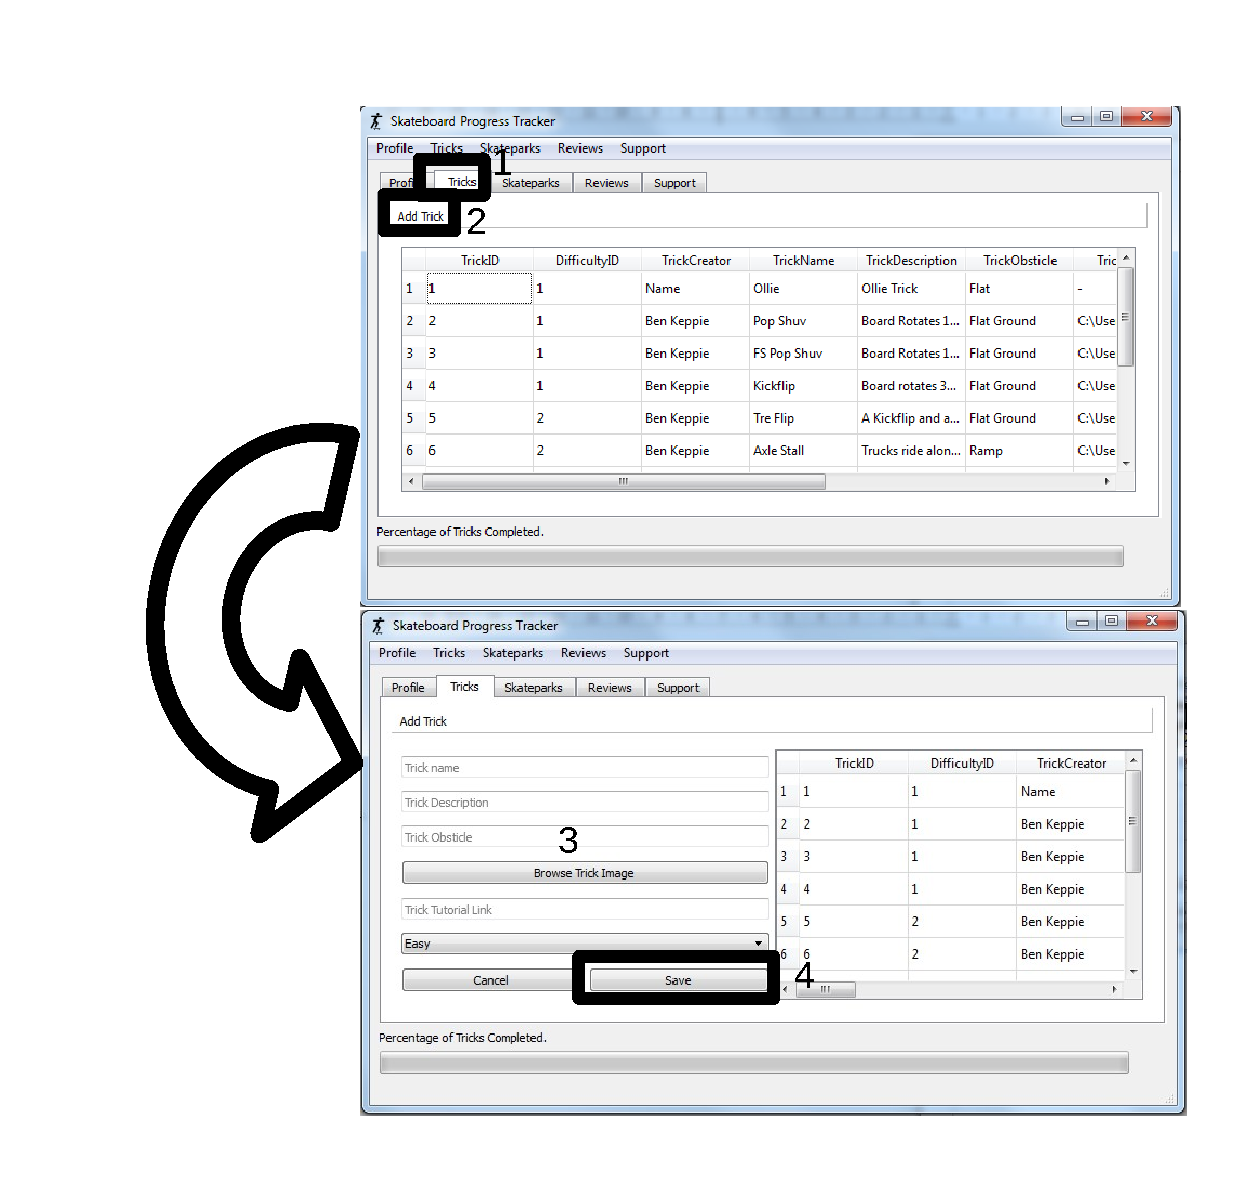
\includegraphics[width=\textwidth]{./Manual/Images/AddTrick.pdf}
    \caption{Adding a Trick} \label{fig:Add Trick}
\end{figure}

The figure above shows you a step by step graphical tutorial in how to change your profile picture. Below, a text tutorial will guide you through the numbers represented on the figure.

\begin{enumerate}
\item Click on the tricks tab.
\item Click on the 'Add Trick' button in the tricks tool bar, this will load a side form allowing you to add details about the trick you wish to add.
\item Fill in all of the fields that you can about that trick. The two optional fields are the trick image and tutorial link.
\item Once you have filled in the information you wish about the trick, click save to add the trick to the database.
\end{enumerate}

\subsubsection{How Do I Delete a Trick?}

\begin{figure}[H]
    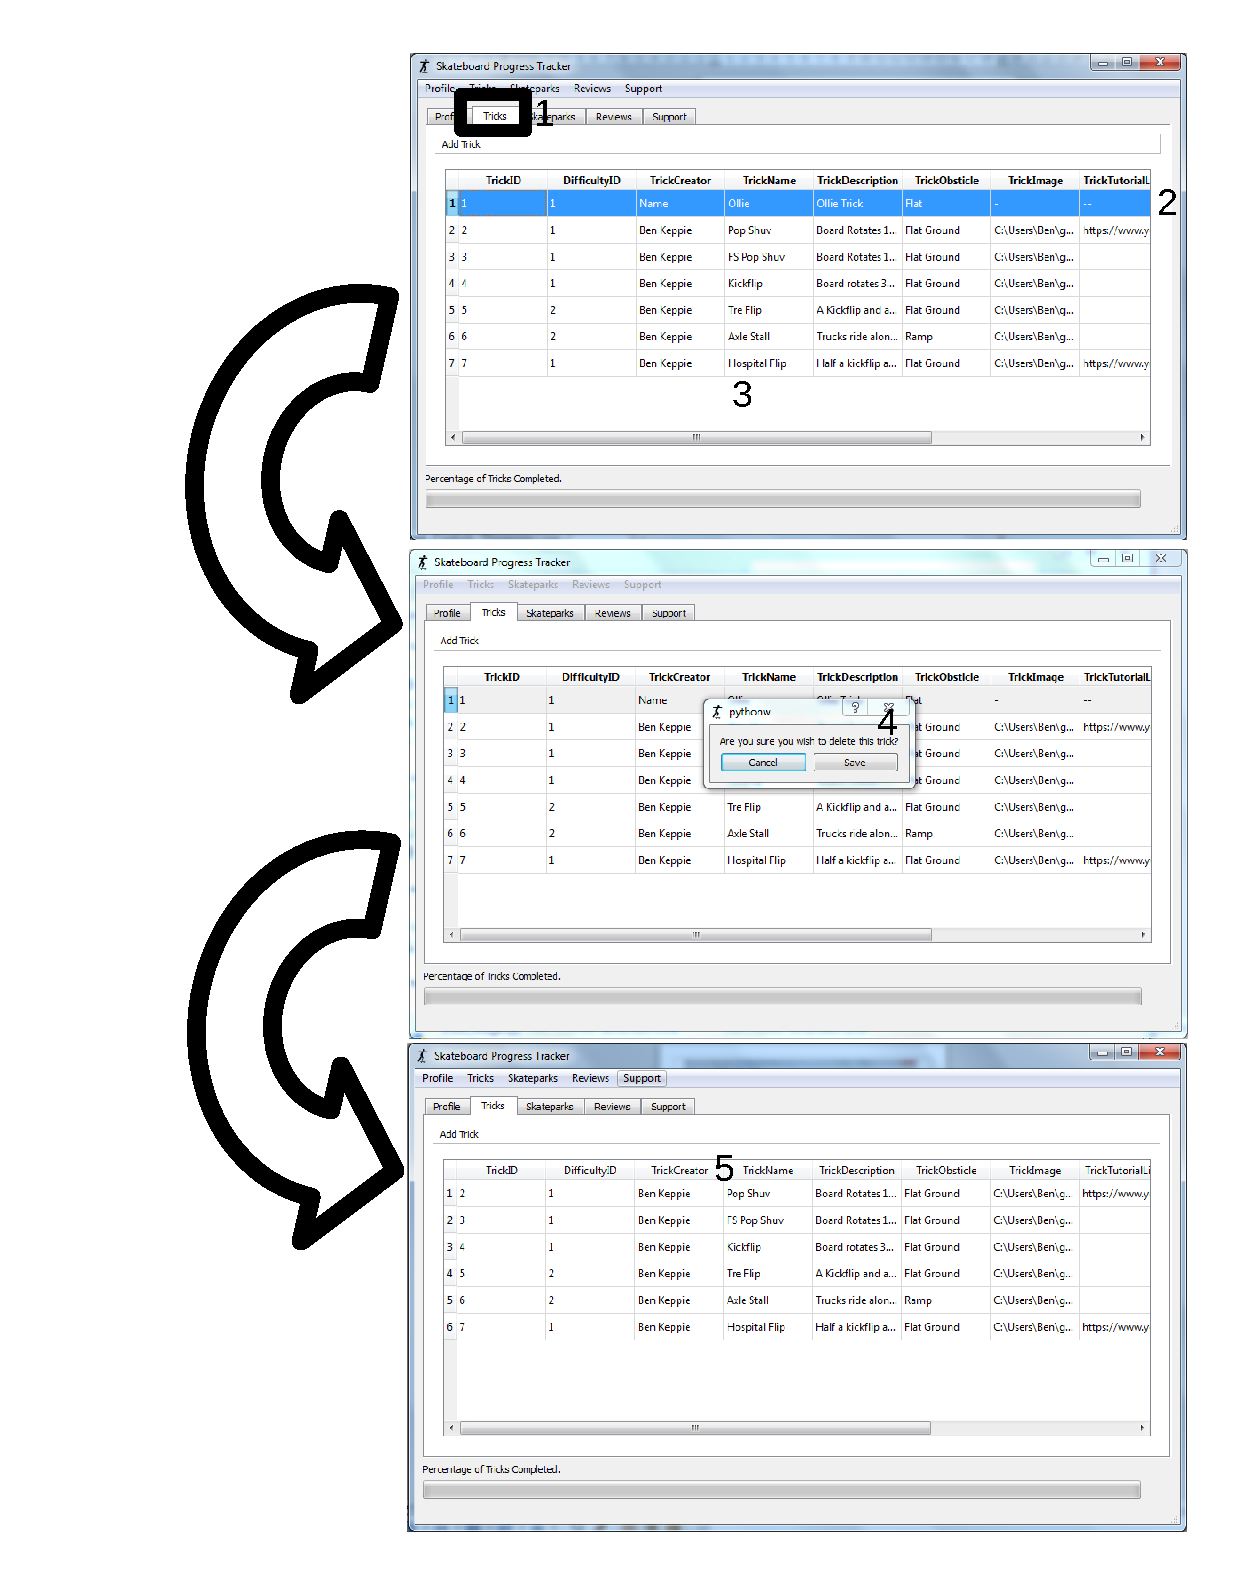
\includegraphics[width=\textwidth]{./Manual/Images/DeleteTrick.pdf}
    \caption{Changing The Profile name} \label{fig:Change Name}
\end{figure}

The figure above shows you a step by step graphical tutorial in how to change your profile picture. Below, a text tutorial will guide you through the numbers represented on the figure.

\begin{enumerate}
\item Click on the 'Tricks' tab.
\item Select the row of the trick that you wish to delete.
\item Press the delete key on your keyboard.
\item Pressing the delete key will stimulate a dialog box to appear, confirming that you wish to delete that trick. To delete the trick click on the save button and to keep the trick press the cancel button.
\item If the delete button is pressed the trick will be removed from the database.
\end{enumerate}

\subsubsection{How Do I Add a Skatepark?}

\begin{figure}[H]
    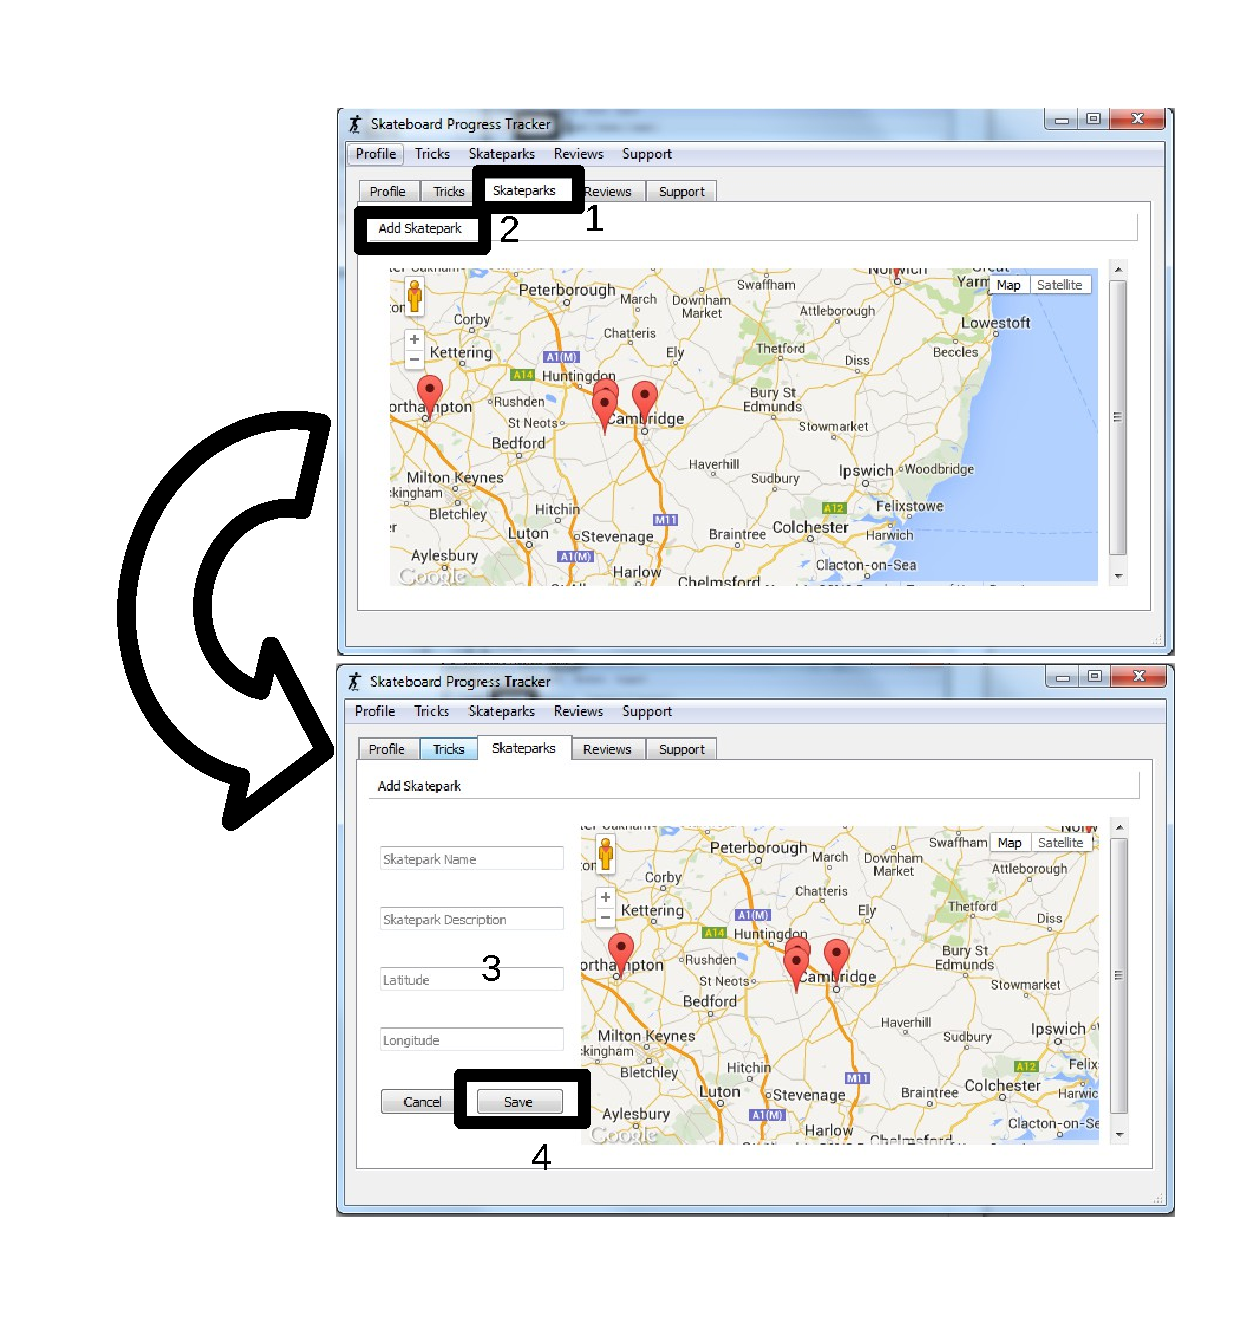
\includegraphics[width=\textwidth]{./Manual/Images/AddSkatepark.pdf}
    \caption{Adding a Skatepark} \label{fig:Add Skatepark}
\end{figure}

The figure above shows you a step by step graphical tutorial in how to change your profile picture. Below, a text tutorial will guide you through the numbers represented on the figure.

\begin{enumerate}
\item Click on the 'Skateparks' tab.
\item Click on the 'Add Skatepark' button in the skateparks tool bar, this will load a side form allowing you to add details about the skatepark you wish to add.
\item Fill in all of the fields that you can about the trick, and then click on the location of the skatepark on the map to fill in the coordinates of the skateparks location.
\item Once all the fields have been filled in, click save to add the skatepark to the database, only the last marker you placed will be saved.
\end{enumerate}

\subsubsection{How Do I Access Existing Skatepark Details?}

\begin{figure}[H]
    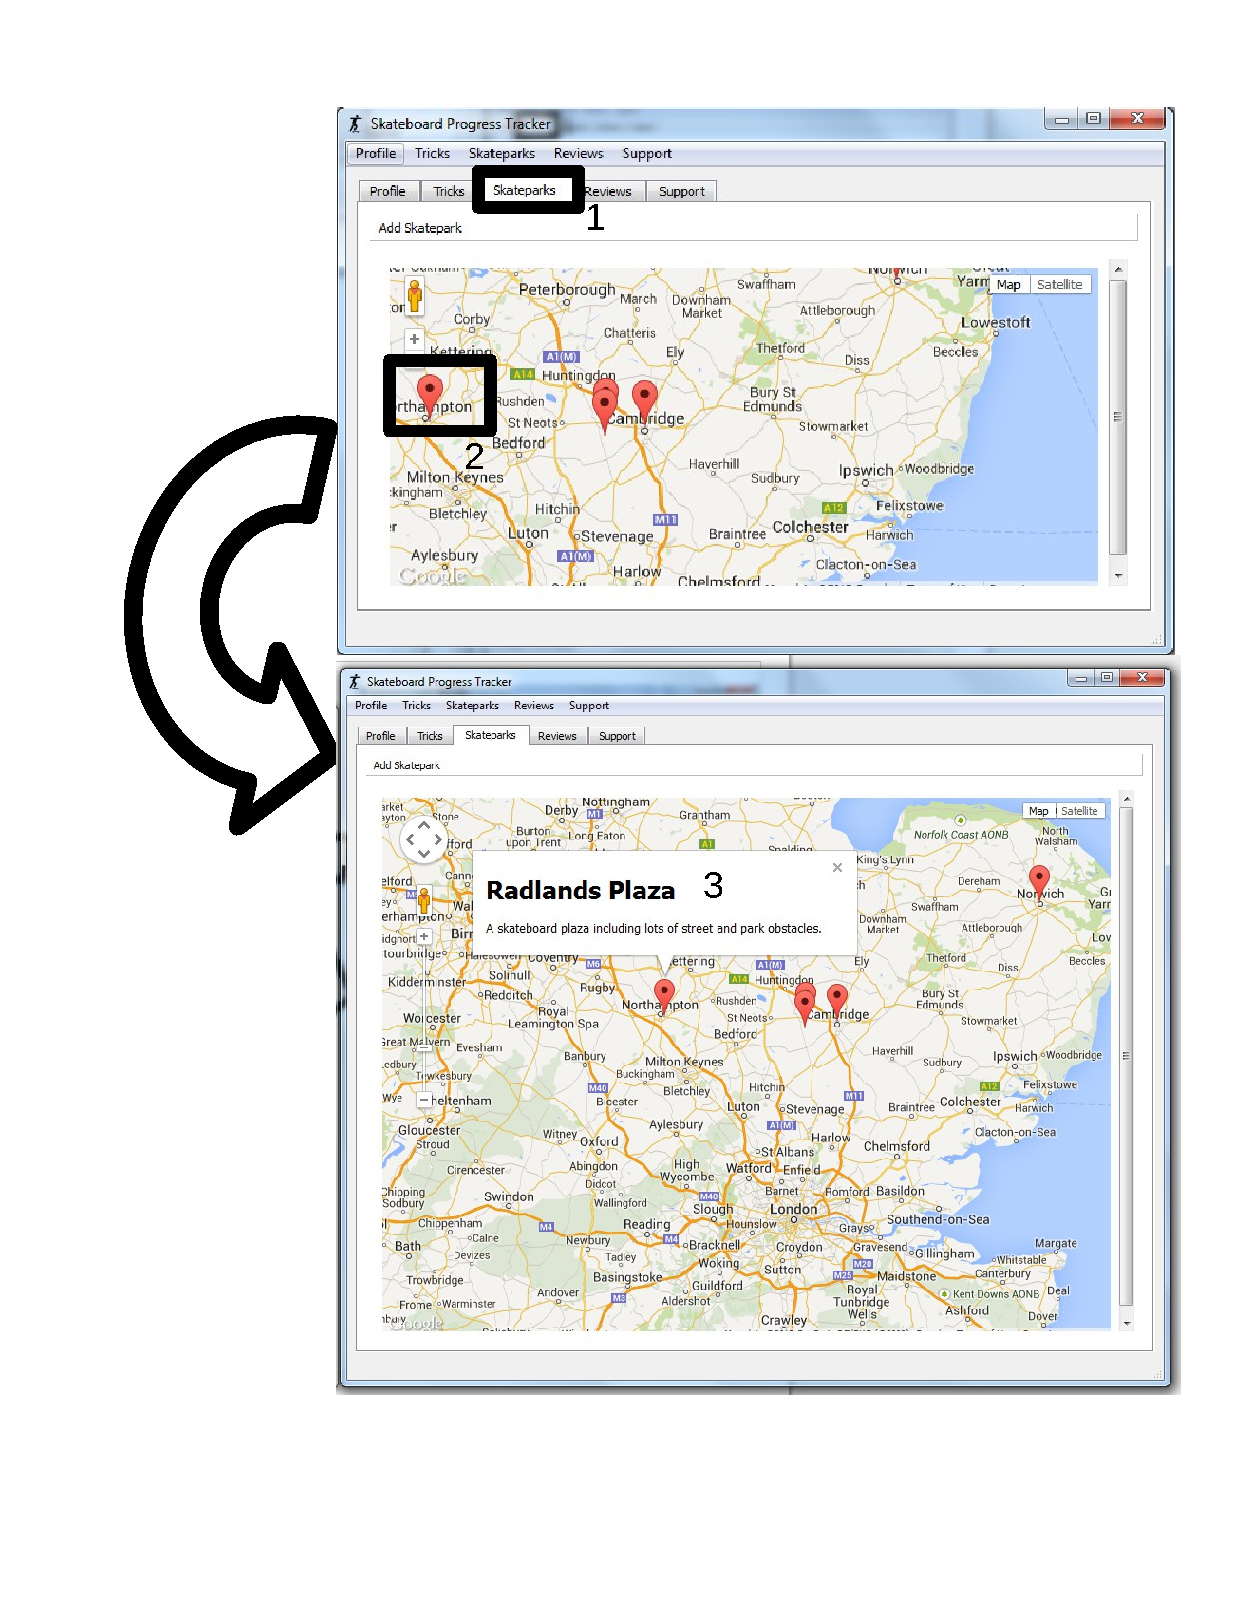
\includegraphics[width=\textwidth]{./Manual/Images/SkateparkDetails.pdf}
    \caption{Accessing Skatepark Details} \label{fig:Skatepark Details}
\end{figure}

The figure above shows you a step by step graphical tutorial in how to change your profile picture. Below, a text tutorial will guide you through the numbers represented on the figure.

\begin{enumerate}
\item Click on the 'Skateparks' tab.
\item Find the marker of the skatepark which you wish to find the details of.
\item Hover your mouse over that marker, and an information window will appear, giving you details about that specific skatepark.
\end{enumerate}

\subsubsection{How Do I Hide Skateparks?} 

\begin{figure}[H]
    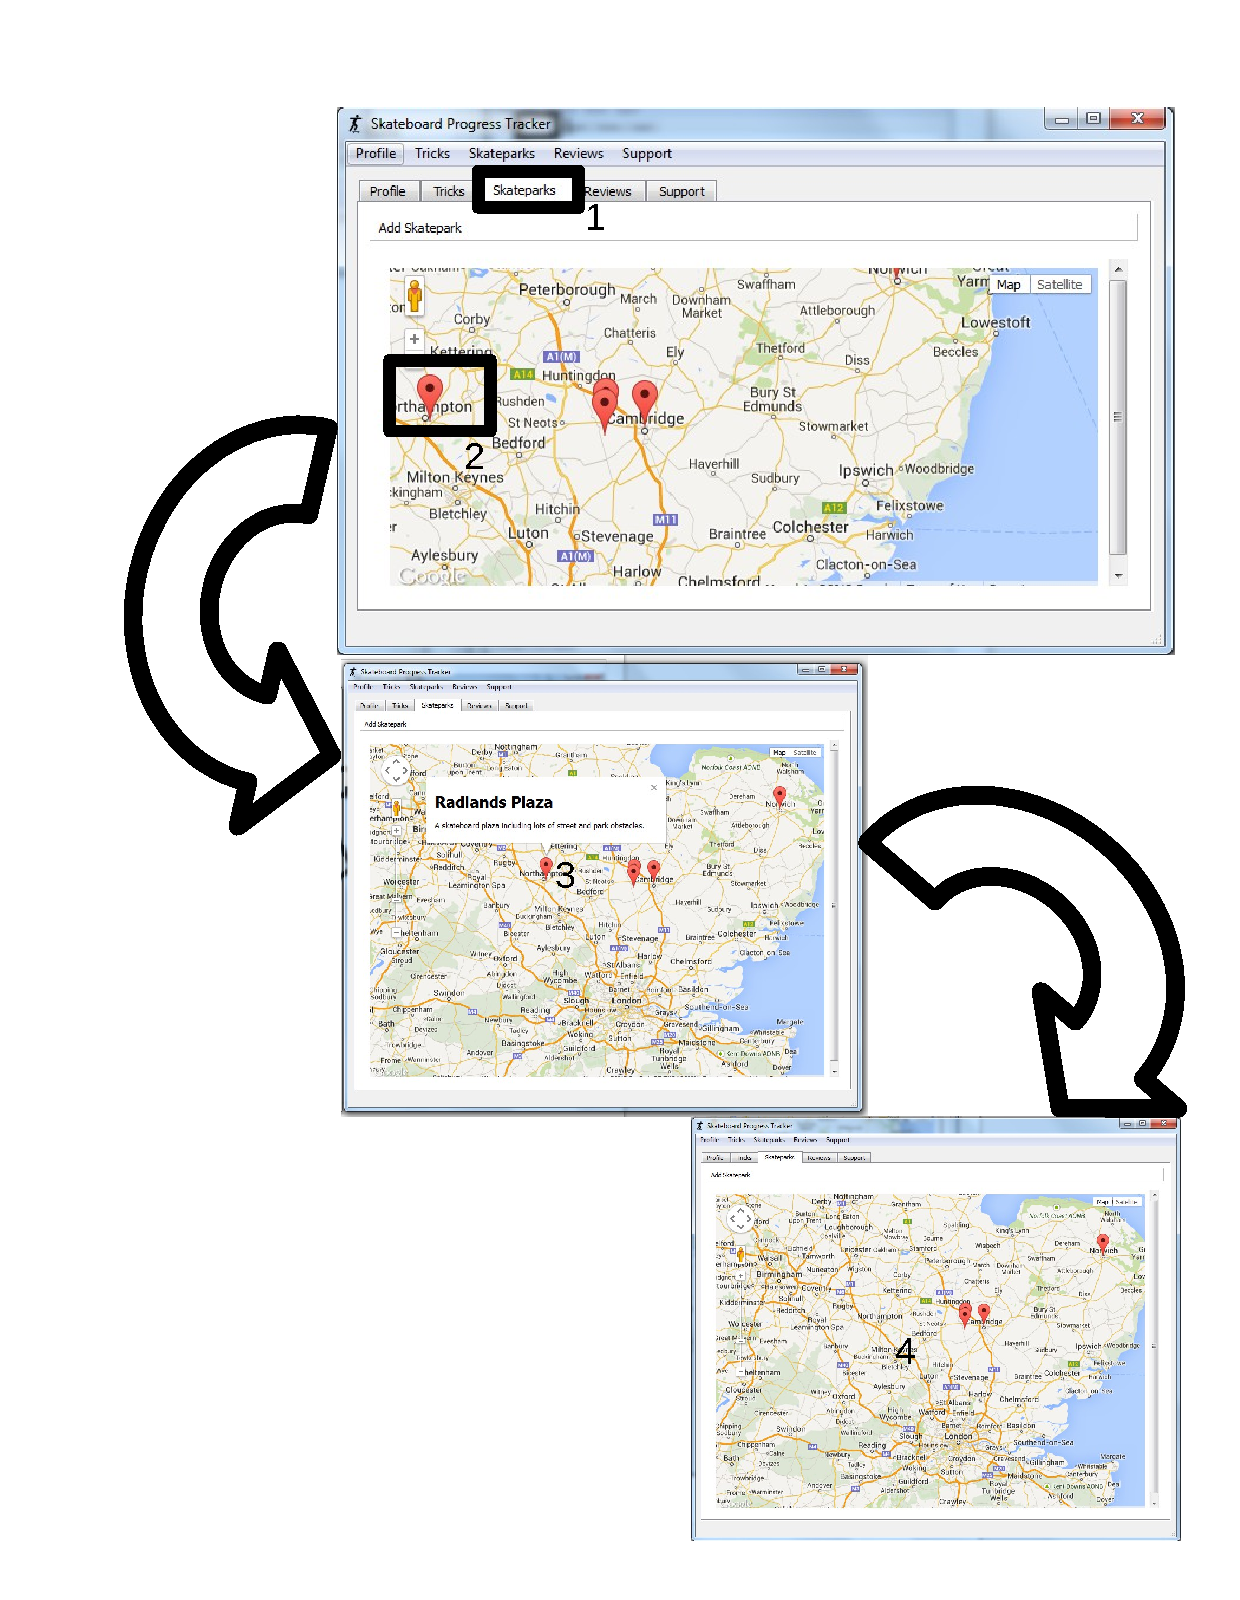
\includegraphics[width=\textwidth]{./Manual/Images/HideSkatepark.pdf}
    \caption{Hiding Skatepark Markers} \label{fig:Hide Skatepark}
\end{figure}

The figure above shows you a step by step graphical tutorial in how to change your profile picture. Below, a text tutorial will guide you through the numbers represented on the figure.

\begin{enumerate}
\item Click on the 'Skateparks' tab.
\item Find the marker of the skatepark which you want to hide.
\item Hover over the skatepark you wish to hide and right click on it.
\item The skatepark is now hidden.
\end{enumerate}



\subsubsection{How Do I Contact Support?}

\begin{figure}[H]
    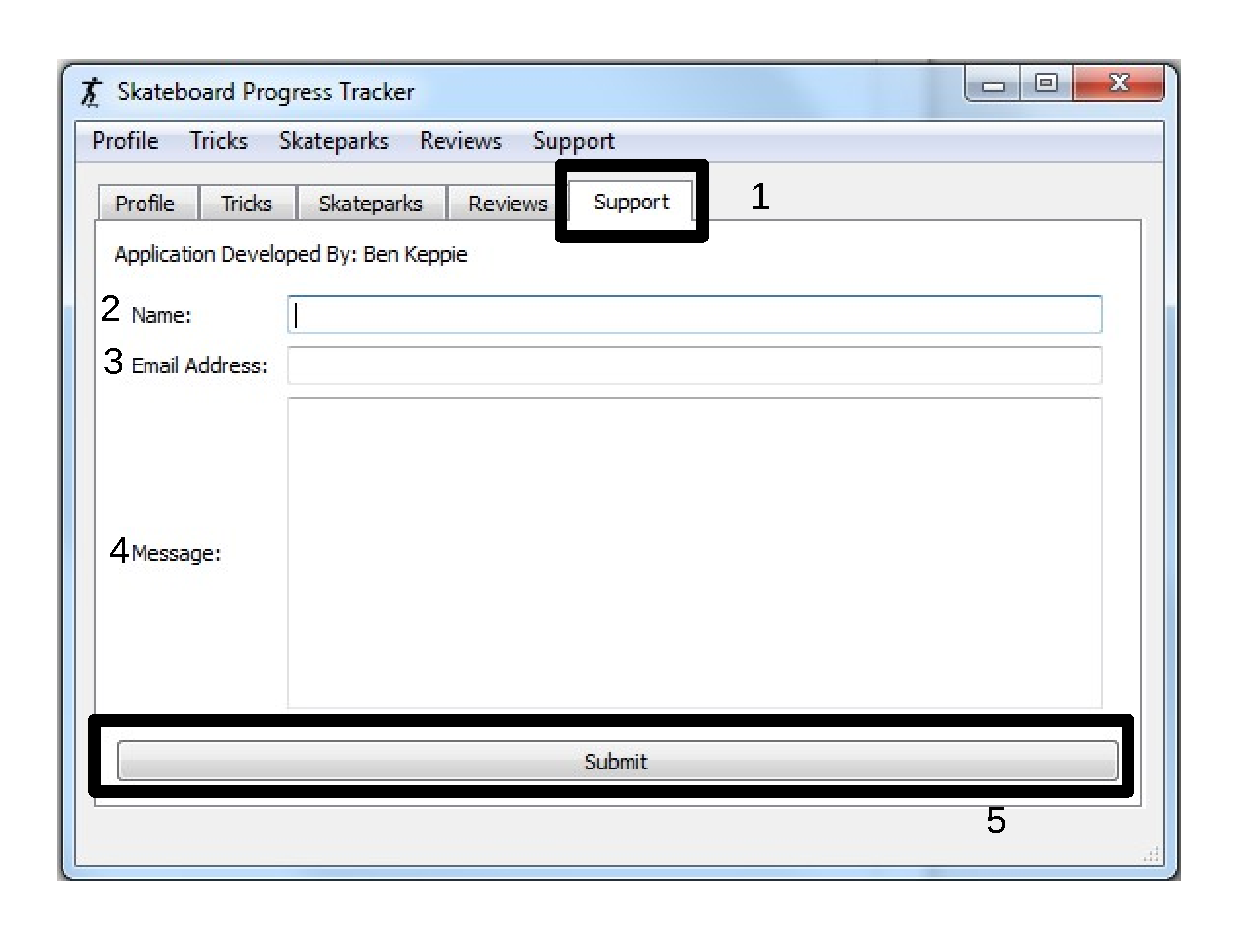
\includegraphics[width=\textwidth]{./Manual/Images/Support.pdf}
    \caption{Contacting Support} \label{fig:Support}
\end{figure}

The figure above shows you a step by step graphical tutorial in how to change your profile picture. Below, a text tutorial will guide you through the numbers represented on the figure.

\begin{enumerate}
\item Click on the 'Support' tab.
\item Fill your name in the field labeled: Name.
\item Fill your Email Address in the field labeled: Email Address.
\item Fill your query in the field labeled: Message.
\item Click the submit button to send your query to the support team.
\end{enumerate}


\textbf{Command Line Interface Tutorials}

For the next tutorials you will need to open up the command line interface menu. This is shown below.

\begin{figure}[H]
    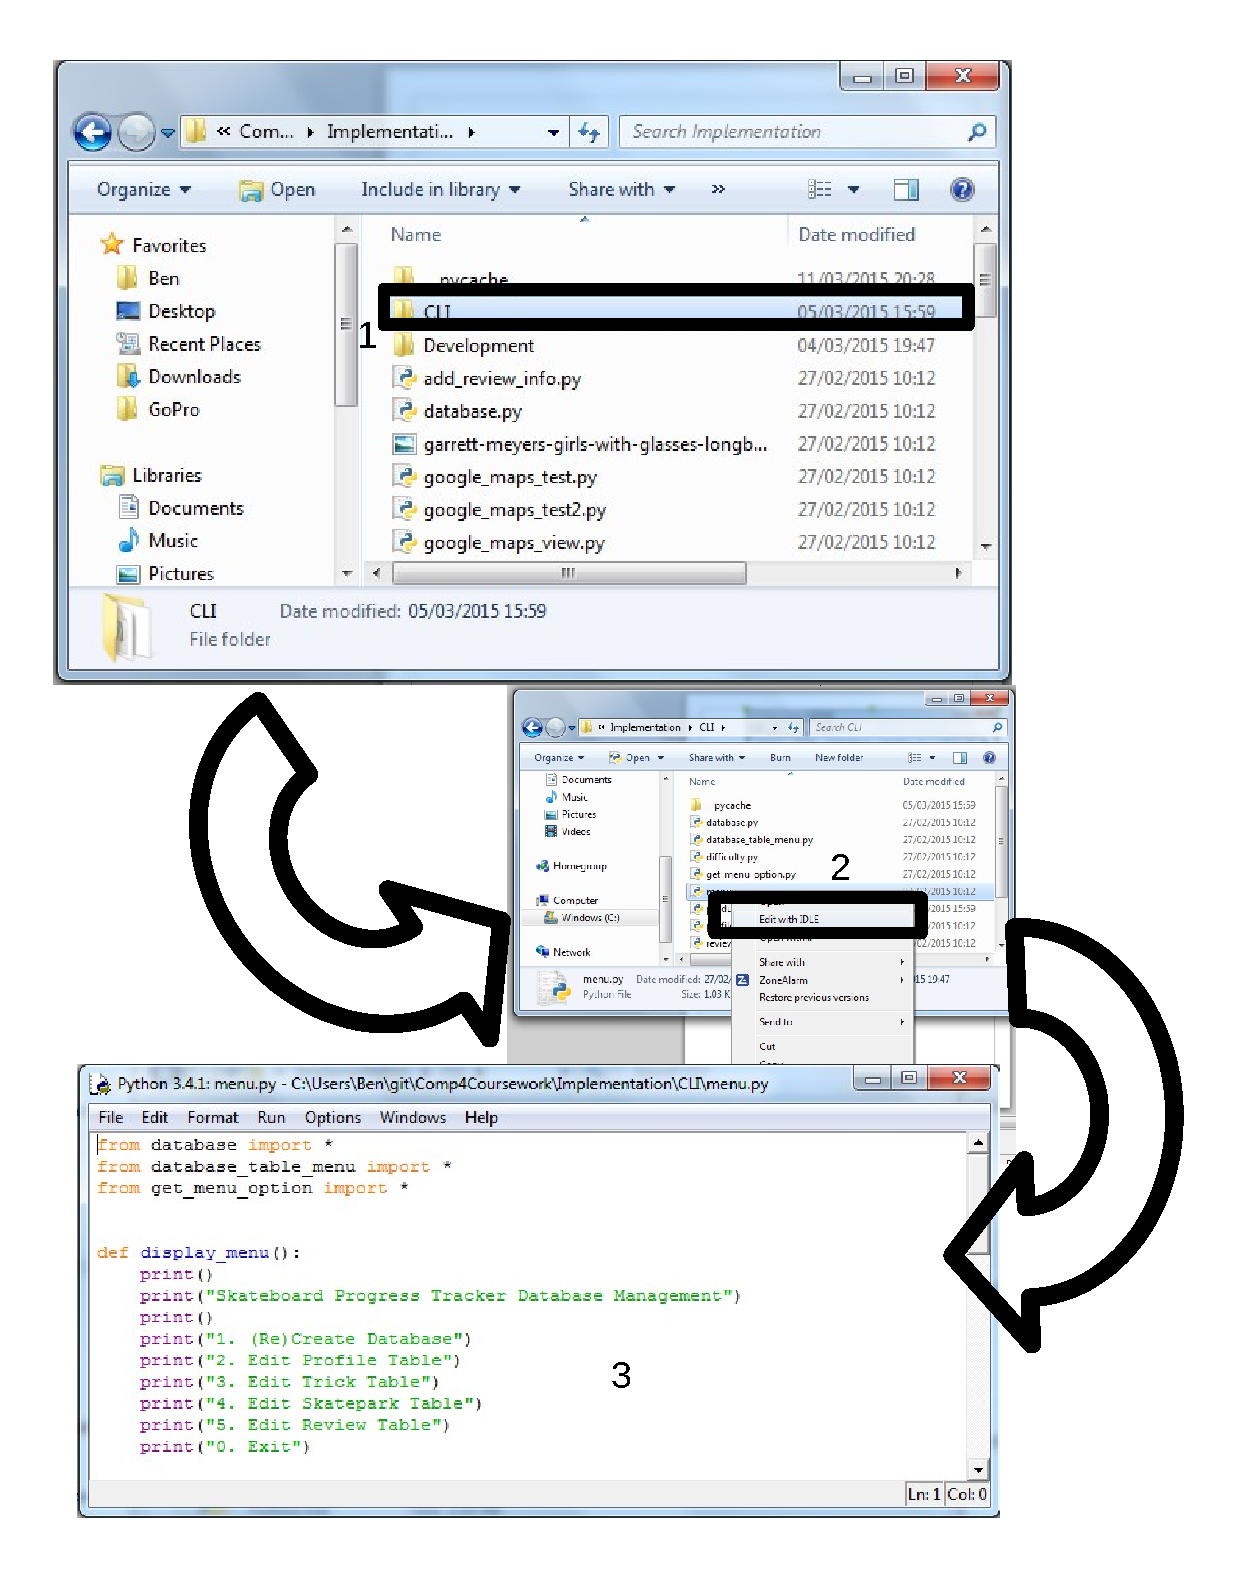
\includegraphics[width=\textwidth]{./Manual/Images/LoadingCLI.pdf}
    \caption{Loading The CLI Menu} \label{fig:Loading CLI}
\end{figure}

\begin{enumerate}
\item Double click the 'CLI' folder.
\item Right click on the file named 'menu.py' and click on the 'Edit with IDLE' option.
\item Press F5 to start up the Command Line Interface.
\end{enumerate}

\subsubsection{How Do I Add a Review?}

The figure below shows the options you need to choose in order to add a review. 

\begin{figure}[H]
    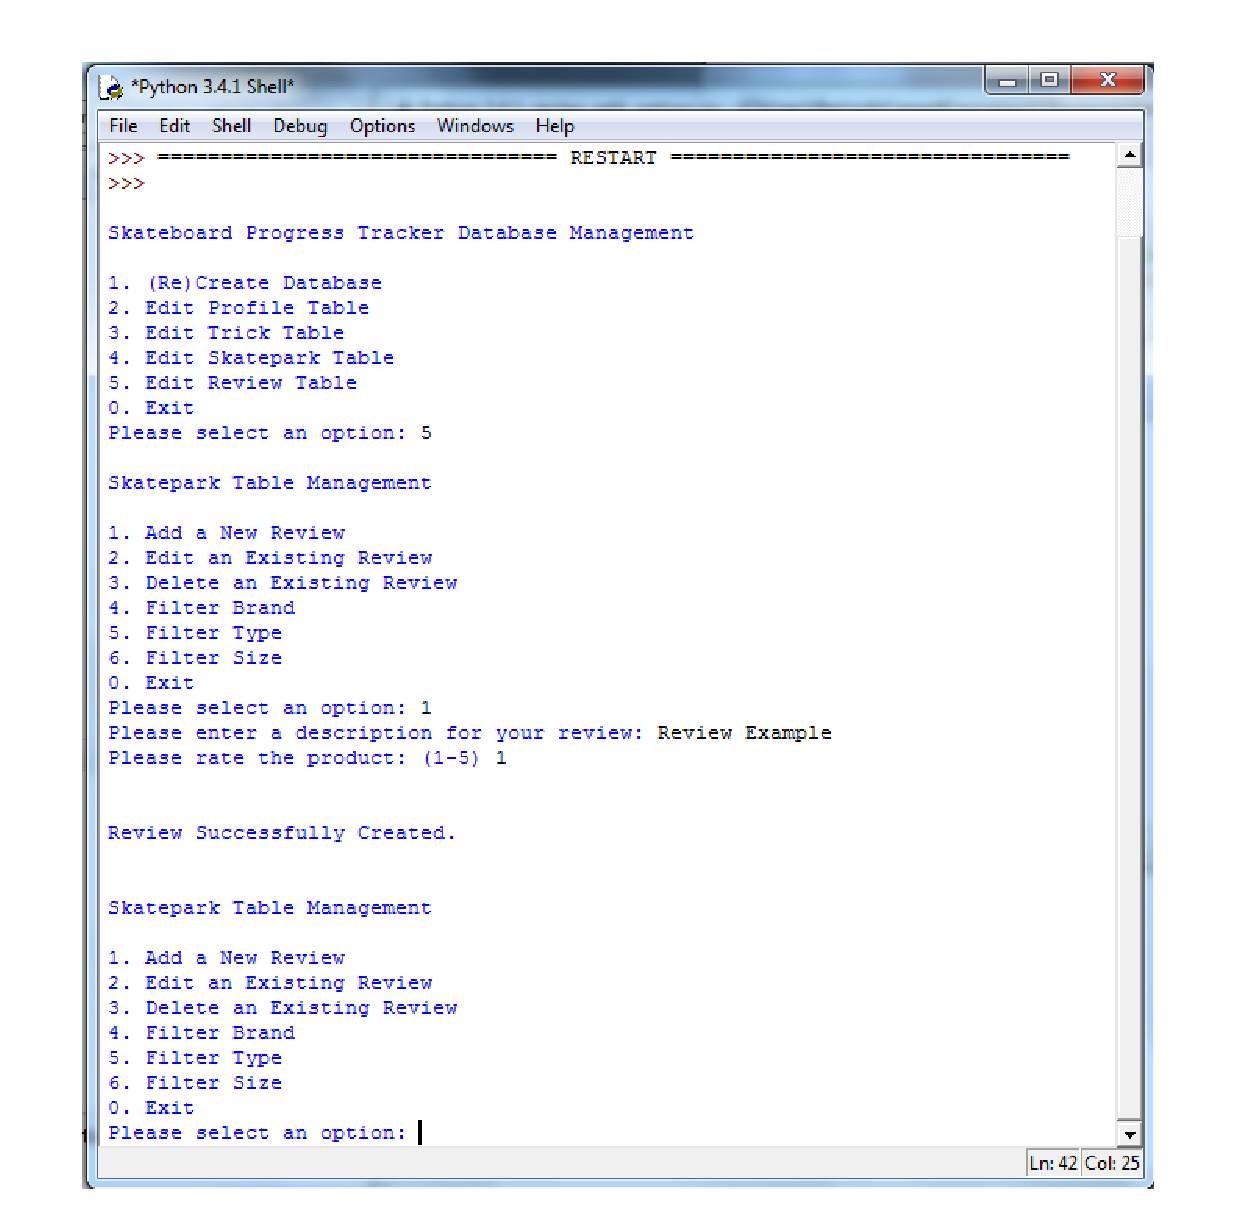
\includegraphics[width=\textwidth]{./Manual/Images/AddReview.pdf}
    \caption{Adding a Review in CLI} \label{fig:Add Review}
\end{figure}



\subsubsection{How Do I Edit a Review?}

The figure below shows the options you need to choose in order to edit a review.

\begin{figure}[H]
    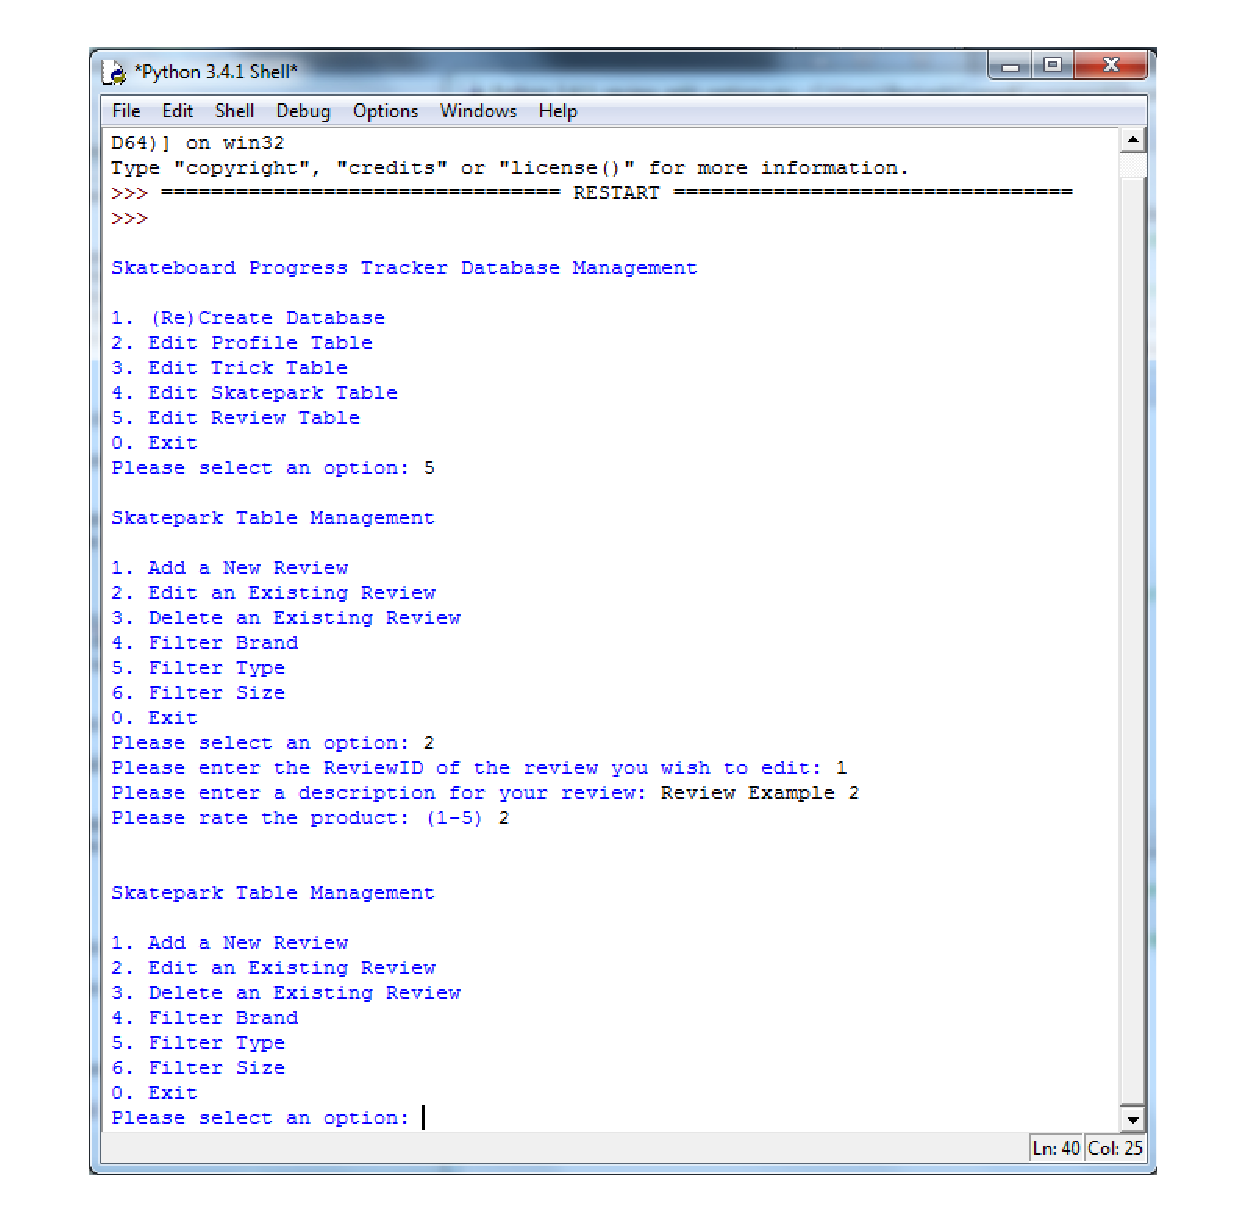
\includegraphics[width=\textwidth]{./Manual/Images/EditReview.pdf}
    \caption{Editing a Review in CLI} \label{fig:Edit Review}
\end{figure}


\subsubsection{How Do I Delete a Review?}

The figure below shows the options you need to choose in order to delete a review.

\begin{figure}[H]
    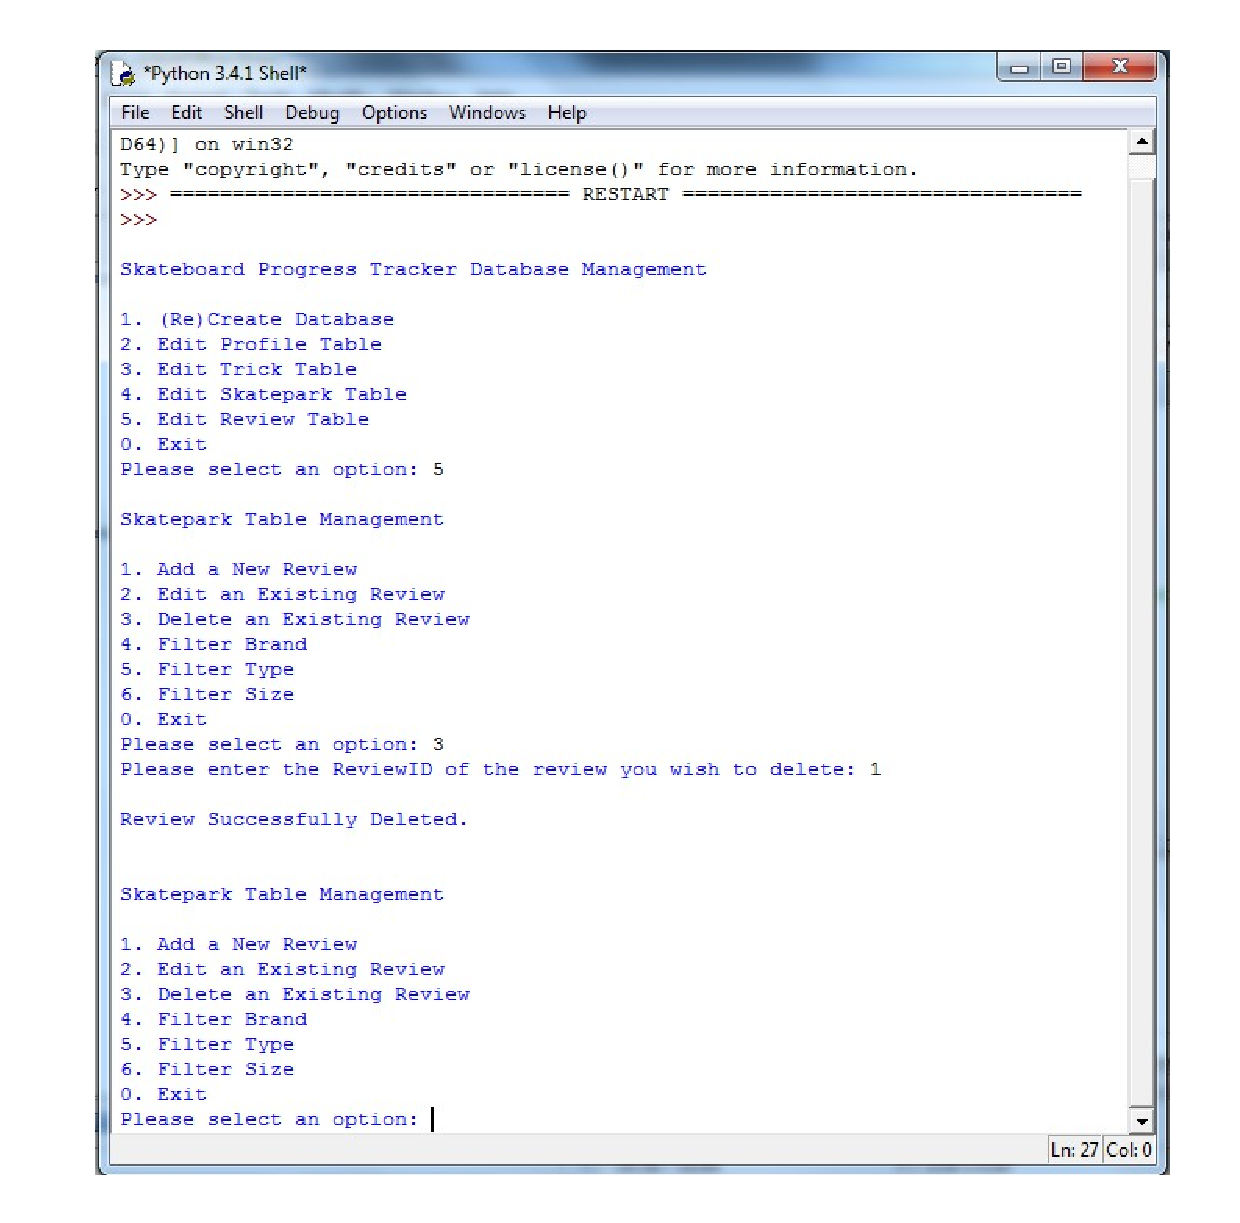
\includegraphics[width=\textwidth]{./Manual/Images/DeleteReview.pdf}
    \caption{Deleting a Review in CLI} \label{fig:Delete Review}
\end{figure}


\subsection{Saving}

My program saves information automatically due to the underlying SQL framework.

\subsection{Limitations}

As discussed in the introduction some sections are not fully implemented into a graphical user interface. This limitation has occurred due to the time limit that I had in order to complete the project.





\section{Error Recovery}

My program contains no errors which lead to the program needing to be recovered in any way.




\section{System Recovery}

\subsection{Backing-up Data}

To back up the program, you need to copy the folder that you extracted during the installation to an external hard drive/USB drive. The figure below shows the backing up of the system to a USB drive.

\begin{figure}[H]
    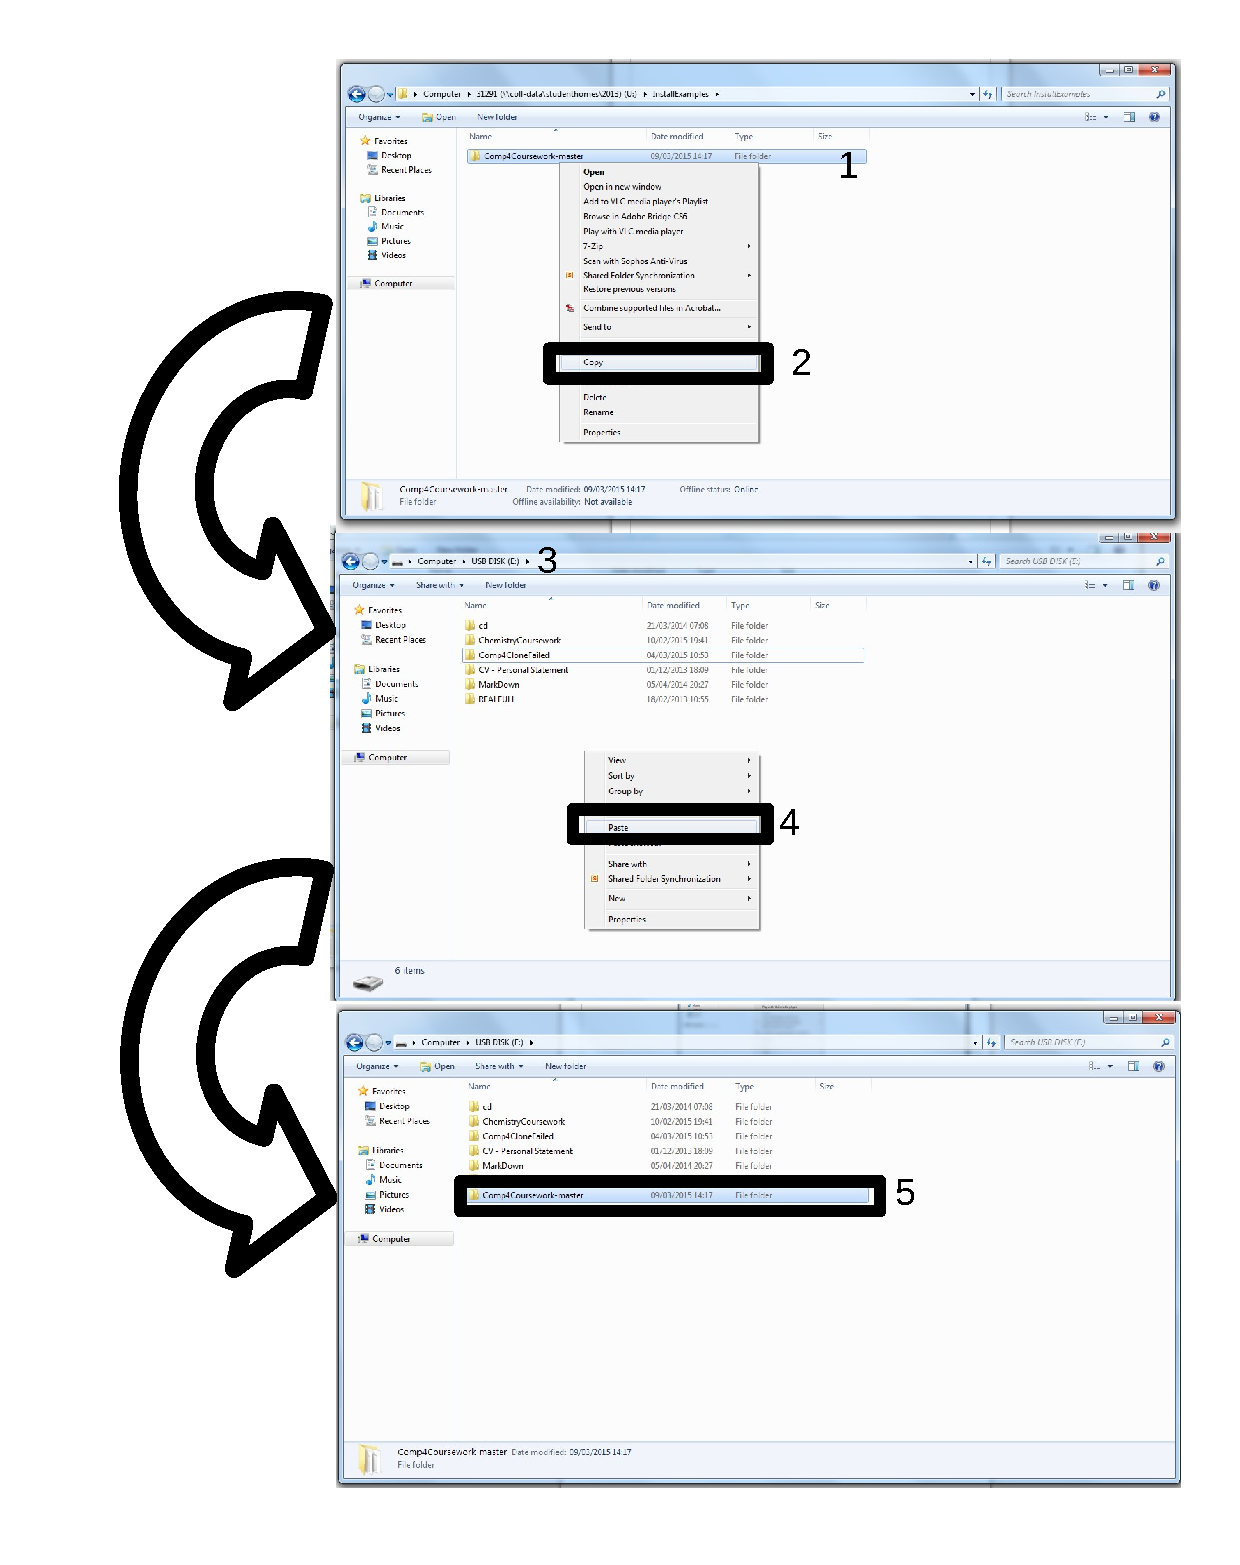
\includegraphics[width=\textwidth]{./Manual/Images/BackUp.pdf}
    \caption{Backing Up The Skateboard Progress Tracker} \label{fig:BackUp}
\end{figure}

\begin{enumerate}
\item Find the location of the folder that you extracted during the installation of the program.
\item Right click on the folder and select 'copy'.
\item Find the USB drive folder and open it.
\item Right click in the folder and select 'paste' 
\item Wait for the copying process to finish, and the back up of the program will be on your USB drive.
\end{enumerate}

\subsection{Restoring Data}

The process for restoring the program data is shown below.

\begin{figure}[H]
    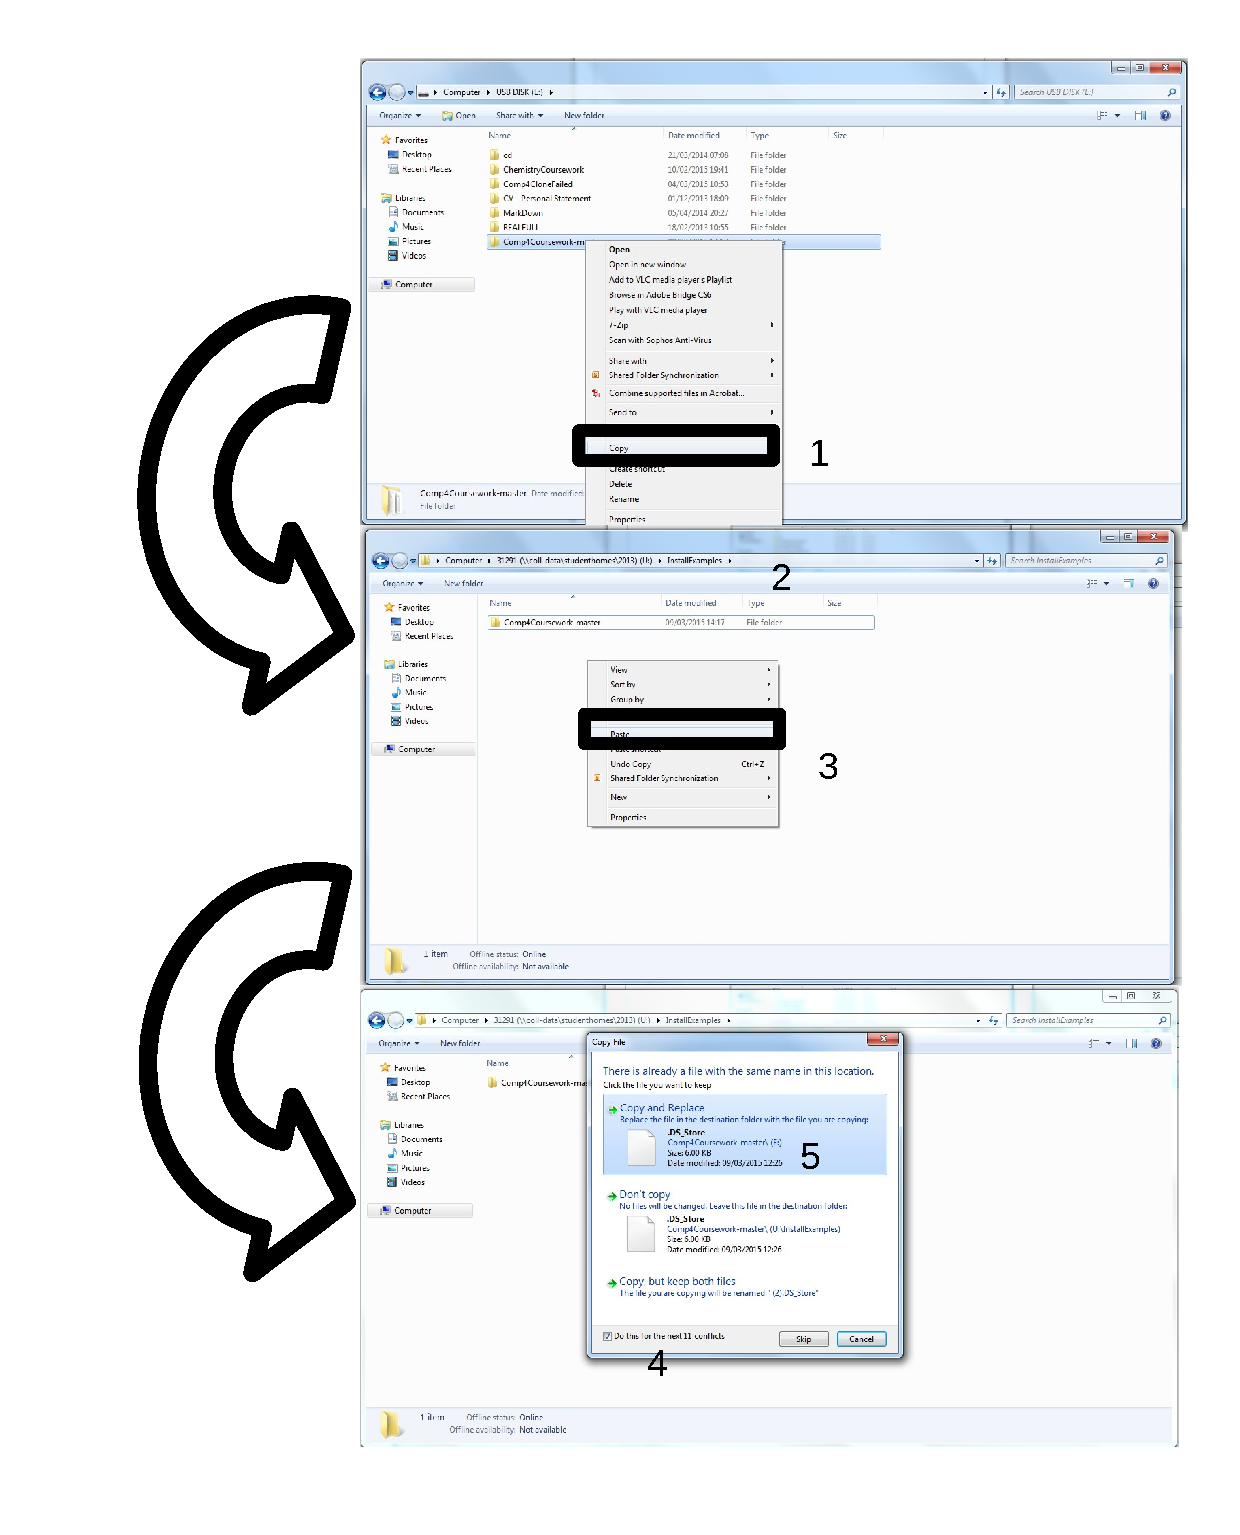
\includegraphics[width=\textwidth]{./Manual/Images/RestoringData.pdf}
    \caption{Restoring The Skateboard Progress Tracker Data} \label{fig:Restoring Data}
\end{figure}

\begin{enumerate}
\item Find the device that you used to back up the program and right click on the folder and press 'copy'.
\item Go to the location of the program on your computer.
\item Right click in the folder location and select 'paste'.
\item Tick the 'Do this for the next X conflicts'.
\item Select copy and replace until the program has been fully replaced.
\end{enumerate}